%---------------------------------------------------------------------------
%
%                          Vorlage der Arbeitsgruppe
%             Computer Vision and Pattern Recognition Group (CVPR)
%                           der Universität Münster
%                         http://cvpr.uni-muenster.de
%
%---------------------------------------------------------------------------
% Geeignet für:
%  - Seminararbeiten
%  - Bachelorarbeiten
%  - Masterarbeiten
%---------------------------------------------------------------------------
% Autoren:
%  - Daniel Tenbrinck
%  - Fabian Gigengack
%  - Michael Schmeing
%  - Lucas Franek
%  - Andreas Nienkötter
%---------------------------------------------------------------------------
% Version:
%  - 1.0.3 (05.10.2016)
%	 - Ersetzung von veralteten Befehlen durch Aktuelle
%	 - Einige ausführlichere Beispiele
%    - Einführung von listings
%    - Aktuelle Version der Eidesstattlichen Erklärung
%  - 1.0.2 (09.09.2011)
%    - Titelblatt um Matrikelnummer und Studiengang ergänzt
%  - 1.0.1 (05.07.2011)
%---------------------------------------------------------------------------
% 
% "THE BEER-WARE LICENSE" (Revision 42):
% The above mentioned authors wrote this file. As long as you retain this
% notice you can do whatever you want with this stuff. If we meet some day,
% and you think this stuff is worth it, you can buy us a beer in return.
%  --------------------------------------------------------------------------

\documentclass[a4paper, twoside, 12pt, ngerman]{scrbook} % Layout-Einstellungen für das Dokument

\usepackage[utf8]{inputenc} % UTF-8 Codierung
\usepackage[ngerman]{babel} % Deutsche Beschriftung
\usepackage{graphicx} % Um Bilder einzufügen
\usepackage{subfigure} % Um mehrere Bilder in eine figure einzufügen
\usepackage{amssymb, amsmath} % Für Mengensymbole und über Gleichheitszeichen schreiben
\usepackage{verbatim} % Um Quellcode in das Dokument einzufügen.
\usepackage{xcolor} % Für Farben
\usepackage[linkbordercolor=blue]{hyperref} % Für Links im Dokument
\usepackage{algorithmic} % Für Pseudo-Code
\usepackage{algorithm} % Wrapper für Pseudo-Code
\usepackage[font={small}, labelfont=bf]{caption} % kleine Bildunterschriften
\usepackage{geometry} % Für Feinanpassungen des Layouts
\usepackage{csquotes} % Um Text in Anführungszeichen zu setzen (\enquote{})
\usepackage{svg} %.svg Bilder einbinden
\usepackage{todonotes} % ToDo-Notizen einfügen
\usepackage{listings} % Für Code-Listings
%\usepackage[style=authortitle-icomp, backend=bibtex]{biblatex}
\renewcommand{\lstlistingname}{Quelltext} %Ändert die Überschrift von Listing nach Quelltext

% Einstellungen für Abstand an den Rändern
\geometry{a4paper,left=35mm,right=35mm,top=20mm,bottom=20mm, includeheadfoot}

\begin{document}
\pagenumbering{roman}
\listoftodos
% Titelblatt
\begin{titlepage}
\begin{centering}
\vspace*{\fill}

\includegraphics[width=12cm]{./img/wwu-logo-neu.pdf}

\vspace{2cm} 

{\LARGE
	\textbf{Untersuchung eines One-vs-One Klassifikationsschemas für tiefe neuronale Netze}\\[1.2cm]
}

{\large
	Bachelorarbeit\\[2cm]
}

{\large
	vorgelegt von:
}

{ \Large
	\textbf{Matthias Carlo Wolff}\\[1cm]
}

{\large
	Matrikelnummer: 458766\\[2mm]
}

{\large
	Studiengang: Informatik\\[1cm]
}
    
{\large
	Thema gestellt von:
}

{\Large
	\textbf{Prof. Dr. Xiaoyi Jiang}\\[1cm]
}
                               
{\large
	Arbeit betreut durch:
}
\todo{Betreut durch wen?}
{\Large
	\textbf{Vorname Nachname}\\[1cm]
}

{\large
Münster, \today
}
\vfill
\end{centering}
\end{titlepage}
% Inhaltsverzeichnis
\tableofcontents

\cleardoublepage
\pagenumbering{arabic}

% Die Hauptkapitel der Arbeit
\chapter{Einleitung}
\label{ch:einleitung}
Diese Bachelorarbeit befasst sich mit dem Thema der sogenannten \textit{One-vs-One} (OvO) Klassifikation in tiefen neuronalen Netzen im Vergleich zu der herkömmlichen \textit{One-vs-All} (OvA) Klassifikation. Als Grundlage für diese Arbeit dient das wissenschaftliche Paper \enquote{One-vs-One classification for deep neural networks} von Pawara et al. \cite{pawaraPaper}.\\

In neuronalen Netzen zur Klassifikation wird fast immer standardmäßig eine OvA Klassifikation angewendet. Die letzte Schicht des Netzes produziert dabei einen Wahrscheinlichkeitsvektor, in dem jeder Klasse eine Wahrscheinlichkeit zugewiesen wird, mit der das Bild zu der jeweiligen Klasse gehört. Alle Wahrscheinlichkeiten zusammen summieren sich dabei zu 100 \% auf. Durch die OvA Klassifikation muss das neuronale Netz lernen, jeweils eine einzige Klasse von allen anderen Klassen gleichzeitig zu unterscheiden und somit genau so viele Klassifikatoren erlernen wie Klassen existieren. Diese Aufgabe ist sehr anspruchsvoll, da komplexe Entscheidungsgrenzen von dem neuronalen Netz erlernt werden müssen (vgl. \cite{pawaraPaper}).\\

Als Alternative zu dem OvA Ansatz existiert das von der \textit{Support-Vector-Machine} bekannte OvO Klassifikationsschema. Bei der OvO Klassifikation werden die Klassen jeweils paarweise voneinander getrennt. Dies ist wesentlich einfacher als eine Klasse von allen anderen gleichzeitig trennen zu müssen, wie es bei der OvA Klassifikation der Fall ist (vgl. \cite{pawaraPaper}).

Hierfür wird in der letzten Schicht anstatt eines Wahrscheinlichkeitsvektors eine Kodierung der Entscheidungen von den einzelnen Klassifikatoren ausgegeben (s. Kapitel \ref{ch:methodik_kodierung}).
Dadurch, dass nun ein Klassifikator jeweils nur zwei Klassen paarweise voneinander trennt, müssen insgesamt mehr Klassifikatoren erlernt werden.
Bei $K$ Klassen müssen für die OvO Klassifikation in dem neuronalen Netz $\frac{K(K-1)}{2}$ Klassifikatoren erlernt werden, bei OvA lediglich $K$ Stück, was besonders bei vielen Klassen, also großem $K$, einen erheblichen Mehraufwand bedeuten kann (vgl. \cite{pawaraPaper}).\\

Da bei der OvO Klassifikation jeweils eine Klasse von nur einer einzigen anderen Klasse abgegrenzt werden muss, wird jeder Klassifikator bei in etwa gleicher Anzahl an Trainingsdaten je Klasse mit einem ausbalancierten Datensatz trainiert. Die Trainingsbeispiele der einen Klasse dienen hierbei als positive und die der anderen Klasse als negative Trainingsbeispiele.
Im Gegensatz dazu wird bei der herkömmlichen OvA Klassifikation jeder Klassifikator mit den Daten einer einzigen Klasse als positive Trainingsbeispiele und mit den Daten der restlichen $K-1$ Klassen als negative Trainingsbeispiele, also einem unbalancierten Datensatz, trainiert (vgl. \cite{pawaraPaper}, 1. Introduction).\\

Daher ist die Motivation bei der Untersuchung eines OvO Klassifikationsschemas ein stabileres Training durch ausbalancierte Trainingsdaten mit denen jeder Klassifikator trainiert wird und eine bessere Performance der Netze durch die weniger komplizierte  Entscheidungsgrenze, die jeder Klassifikator erlernen muss.\\

Um diesen vielversprechenden aber bisher selten benutzten Ansatz der OvO Klassifikation im Vergleich zu der herkömmlichen OvA Klassifikation zu untersuchen, wurden im Paper von Pawara et al. \cite{pawaraPaper} verschiedene Datensätze (s. Kapitel \ref{ch:methodik_datensaetze}) mit verschiedenen Parametern (s. Kapitel \ref{ch:methodik_parameter}) sowohl mit der OvO als auch mit der OvA Klassifikation trainiert und ausgewertet.
Die Autoren kommen zu dem Fazit, dass der OvO Ansatz in 37 von 100 Experimenten signifikant besser ist als der herkömmliche OvA Ansatz und niemals signifikant schlechter wenn die Netze von Grund auf trainiert werden und keine vor-trainierten Gewichte verwendet werden (vgl. \cite{pawaraPaper}, 5.7 Discussion).\\

In dieser Arbeit werden die gleichen Experimente wie im Paper von Pawara et al. \cite{pawaraPaper} durchgeführt und ausgewertet, um die dort erzielten Ergebnisse zu verifizieren. Außerdem werden darüber hinaus noch weitere Experimente angestellt (s. Kapitel \ref{ch:methodik}) und die Ergebnisse anschaulich visualisiert (s. Kapitel \ref{ch:ergebnisse}).\\

Durch die verschiedenen Kombinationen von Parametern müssen sehr viele verschiedene neuronale Netze trainiert werden. Dazu wurden mit Hilfe des High-Performance-Computing Clusters \textit{Palma II} der Universität Münster \cite{palma2} insgesamt 10.070 neuronale Netze trainiert und insgesamt ca. 6.900 GPU Stunden Rechenzeit benötigt (s. Kapitel \ref{ch:methodik_palma}).\\

Sämtlicher Quellcode, der zum Training, Vorbereiten der Datensätze und zum Erstellen der k-Fold Cross Validation benutzt wurde, sowie die tatsächlich verwendete Einteilung der Datensätze und die erzielten Ergebnisse befinden sich in dem zu dieser Arbeit gehörenden GitHub Repository \footnote{\url{https://github.com/M-Wolff/Bachelorarbeit_OvO-Klassifikation}} \cite{githubRepo}.

\chapter{Methodik}
\label{ch:methodik}
\todo{deutlich machen, was ich anders gemacht habe als Pawara und wieso}
\todo{generelles Verfahren in eigenen Worten beschreiben}

\section{OvO-Kodierung}
\label{ch:methodik_kodierung}
\todo{Umsetzung: OvO Matrix, Kodierung, Klassifizierung, eigene Loss-Funktion, softmax vs tanh}
\todo{Warum Datensätze mit 3 Klassen verwendet wurden}

\subsection{Alternative Kodierungsmethoden}
\todo{alternative Kodierungsmöglichkeiten beschreiben (s. Paper, z.B. Error correcting codes)}

\newpage
\section{Datensätze}
\label{ch:methodik_datensaetze}
Für die Experimente wurden 5 verschiedene Datensätze verwendet: Agrilplant \cite{pawaraWebsiteDatensaetze}, Cifar \cite{cifar10}, Monkey \cite{pawaraWebsiteDatensaetze}, SwedishLeaves \cite{swedishLeaves} und Tropic \cite{pawaraWebsiteDatensaetze}.

Für jeden Datensatz existieren Exemplare mit verschiedenen Anzahlen an Klassen (s. Abb. \ref{fig:DatensatzKlassen}), die zukünftig jeweils mit $<$Datensatzname$><$Klassenanzahl$>$ wie z.B. Agrilplant10 bezeichnet werden.
Die Datensätze mit geringerer Klassenanzahl sind Teilmengen des gesamten Datensatzes, bei denen nur die ersten $k$ Klassen verwendet werden.

Bei allen Datensätzen außer SwedishLeaves (s. Kapitel \ref{ch:methodik_SwedishLeaves}) wird eine 5-Fold Cross Validation angewendet, es werden also 5 Aufteilungen in Train- und Testdaten im Verhältnis 80:20 erstellt, sodass sich jedes Bild genau in einem Fold im Testsplit und in 4 Folds im Trainsplit befindet.

Für die Datensätze Tropic10 und Monkey10 stehen auf der Homepage der Autorin \cite{pawaraWebsiteDatensaetze} die von ihr verwendeten Einteilungen in 5 Folds zur Verfügung. Diese Datensätze, die mit der exakt gleichen Einteilung in 5 Folds verwendet wurden, werden im weiteren Verlauf dieser Arbeit mit dem Präfix\\ \enquote{Pawara-} kenntlich gemacht. Da die gleiche Einteilung in 5 Folds verwendet wurde wie im Paper von Pawara et al. \cite{pawaraPaper} ist die Vergleichbarkeit der reproduzierten Ergebnisse höher.

Für alle anderen Datensätze musste die Einteilung in 5 bzw. für SwedishLeaves 3 Folds neu erstellt werden.
Außerdem wurde für Tropic10 ebenfalls eine eigene 5-Fold Cross Validation erstellt, da die von der Autorin zur Verfügung gestellte Einteilung (s. \cite{pawaraWebsiteDatensaetze}) fehlerhaft ist. Ihre sogenannte 5-Fold Cross Validation besteht bei Tropic10 vermutlich aus fünfmaligem, zufälligem Ziehen eines Verhältnisses 70:30 für Trainings und Testdaten. Dies führt dazu, dass ein eventuell schwierig zu klassifizierendes Bild in mehr als einem Fold im Testsplit vorkommen und somit das Ergebnis abhängig vom Zufall beeinflussen kann.
\todo{In Scatterplots schauen, inwiefern diese Aussage stimmt}

\begin{figure}[H]
\begin{tabular}{|c|c|c|c|c|c|}
\hline 
Anzahl an Klassen & 3 & 5 & 10 & 15 & 20 \\ 
\hline 
Agrilplant & X & X & X &  &  \\ 
Cifar &  &  & X &  &  \\ 
Monkey &  &  & X &  &  \\ 
SwedishLeaves & X & X & X & X &  \\ 
Tropic & X & X & X & & X \\ 
\hline 
\end{tabular} 
\caption{Zum Training verwendete Anzahl an Klassen je Datensatz}
\label{fig:DatensatzKlassen}
\end{figure}

\subsection{Agrilplant}
Der Agrilplant Datensatz \cite{pawaraWebsiteDatensaetze} besteht aus Bildern von Blüten, Früchten und Blättern von Agrarpflanzen.
Es existieren 10 verschiedene Klassen: Apfel, Banane, Traube, Jackfruit, Orange, Papaya, Kaki, Ananas, Sonnenblume und Tulpe (vgl. \cite{pawaraWebsiteDatensaetze}).
\begin{figure}[H]
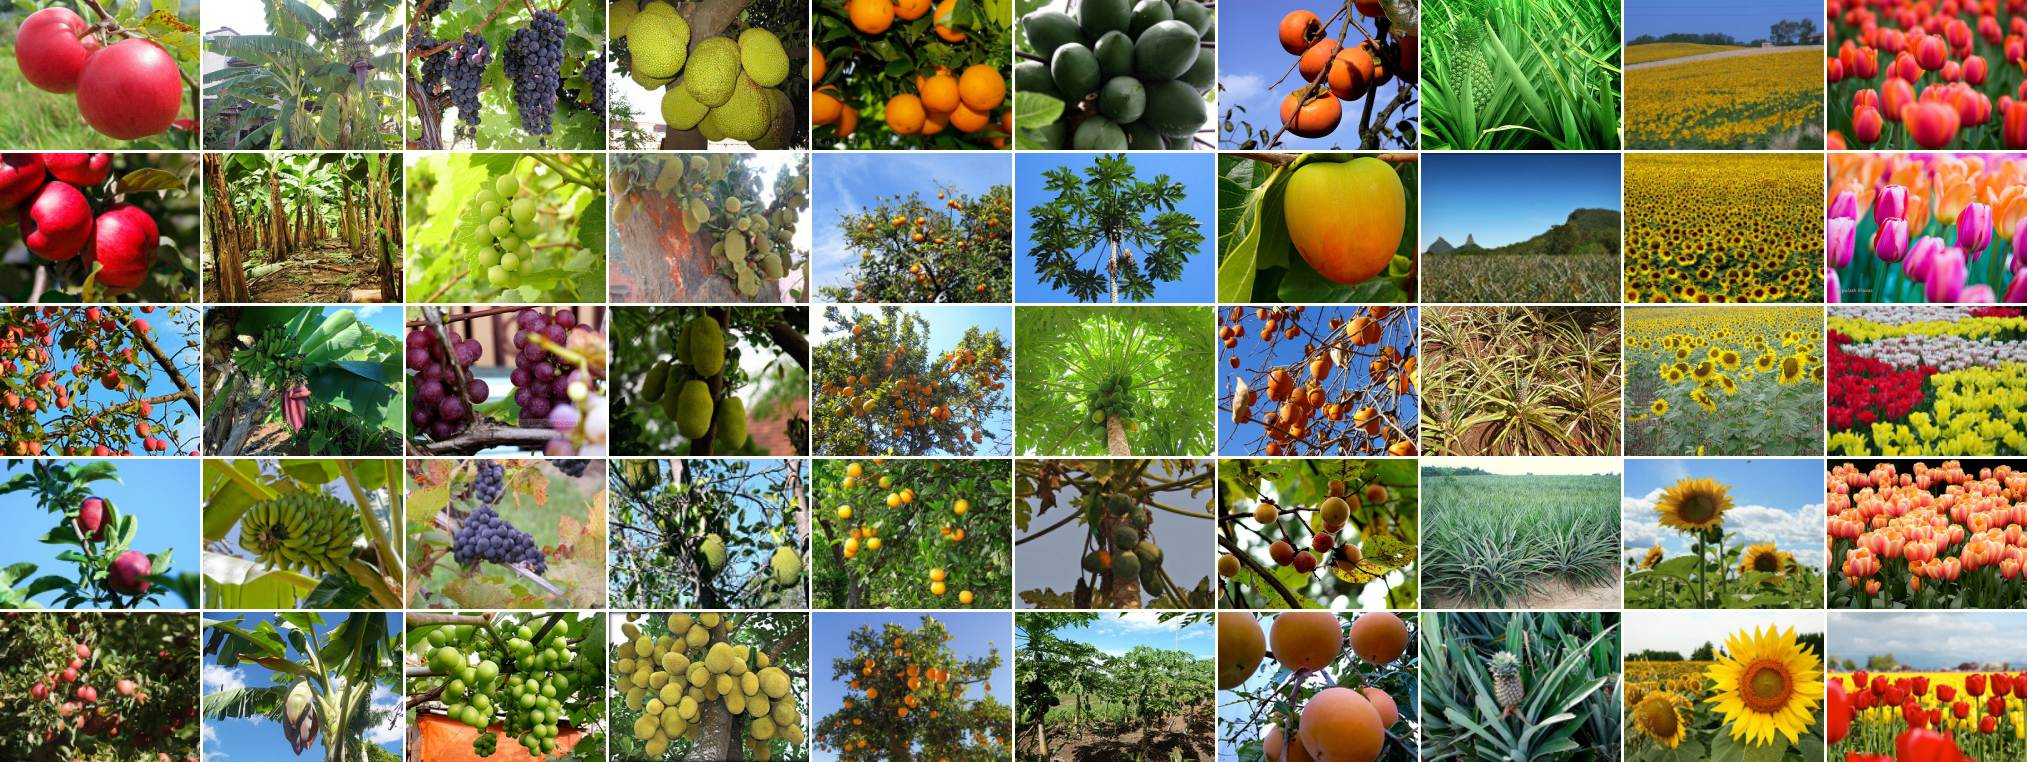
\includegraphics[scale=0.2]{img/2_agrilplant-image.jpg}
\caption{Überblick über die verschiedenen Klassen des Agrilplant Datensatzes \cite{pawaraAgrilplant}.}
\label{fig:agrilplantUeberblick}
\end{figure}

Zum Training wurden zusätzlich zu Agrilplant10 noch zwei weitere Teilmengen des Datensatzes, Agrilplant5 und Agrilplant3, verwendet.

Der Datensatz Agrilplant10 besteht aus 300 Bildern mit einer Auflösung von ca. 200-500 Pixeln je Klasse, also insgesamt 3000 Bilder, und ist damit perfekt ausbalanciert (s. Abb. \ref{fig:Agrilplant10Zusammensetzung}).\\


\begin{figure}[H]
\begin{adjustbox}{width=1.4\textwidth, center}
\includesvg{img/2_agrilplant10_Zusammensetzung}
\end{adjustbox}
\caption{Aufteilung des Agrilplant10 Datensatzes \cite{pawaraWebsiteDatensaetze} in Train- und Testsplits je Fold.}
\label{fig:Agrilplant10Zusammensetzung}
\end{figure}


\subsection{Cifar}
Der Cifar10 Datensatz beinhaltet insgesamt 60.000 Bilder in einer sehr kleinen Auflösung von 32x32 Pixeln. Es existieren 10 Klassen: Flugzeug, Automobil, Vogel, Katze, Hirsch, Hund, Frosch, Pferd, Schiff, Lastkraftwagen (vgl. \cite{cifar10}).
Die Aufteilung in Klassen ist perfekt ausbalanciert mit genau 6.000 Bildern pro Klasse (s. Abb. \ref{fig:Cifar10Zusammensetzung}).
Da die zum Training verwendeten Netze für Bilder in einer Auflösung von 224 bzw. 299 Pixeln ausgelegt sind (vgl. \ref{ch:methodik_netze}) müssen die Bilder von diesem Datensatz ungefähr 8-fach vergrößert werden.\\

Durch die große Anzahl an Bildern und die starke Hochskalierung benötigt das Training viel Zeit und Ressourcen, weshalb Cifar10 nur bei Resnet Scratch verwendet wird.
\todo{Verlinkung setzen auf Trainingsdauer, Aussage wie viel länger als z.B. Tropic20}

Dieser Datensatz wurde zusätzlich zu den anderen ausgewählt um die Aussagekraft der Ergebnisse zu erhöhen, da sich die anderen Datensätze lediglich auf Pflanzen und Affen beschränken. Im wissenschaftlichen Paper von Pawara et al. \cite{pawaraPaper} wird dieser Datensatz nicht behandelt.

\begin{figure}[H]
\begin{adjustbox}{width=1.4\textwidth, center}
\includesvg{img/2_cifar10_Zusammensetzung}
\end{adjustbox}
\caption{Aufteilung des Cifar10 Datensatzes \cite{cifar10} in Train- und Testsplits je Fold.}
\label{fig:Cifar10Zusammensetzung}
\end{figure}


\subsection{Monkey}
Für den Monkey Datensatz existieren 2 Versionen: Pawara-Monkey10 und Pawara-uMonkey10 mit absichtlich nicht ausbalancierten Anzahlen an Bildern je Klasse, um zu untersuchen wie die beiden Klassifikationsschemata auf schlecht ausbalancierten Datensätzen abschneiden (vgl. \cite{pawaraWebsiteDatensaetze}). Beide Versionen bestehen aus Bildern aus 10 Klassen von verschiedenen Affenarten aufgenommen in freier Wildbahn aus unterschiedlichen Perspektiven (s. Abb. \ref{fig:monkey10Ueberblick}) und wurden in genau der gleichen Aufteilung in Folds bei den Experimenten im Paper von Pawara et al. \cite{pawaraPaper} verwendet.
Die Bilder haben eine Auflösung von ca. 180 bis zu 6.000 Pixeln.
\begin{figure}[H]
\centering
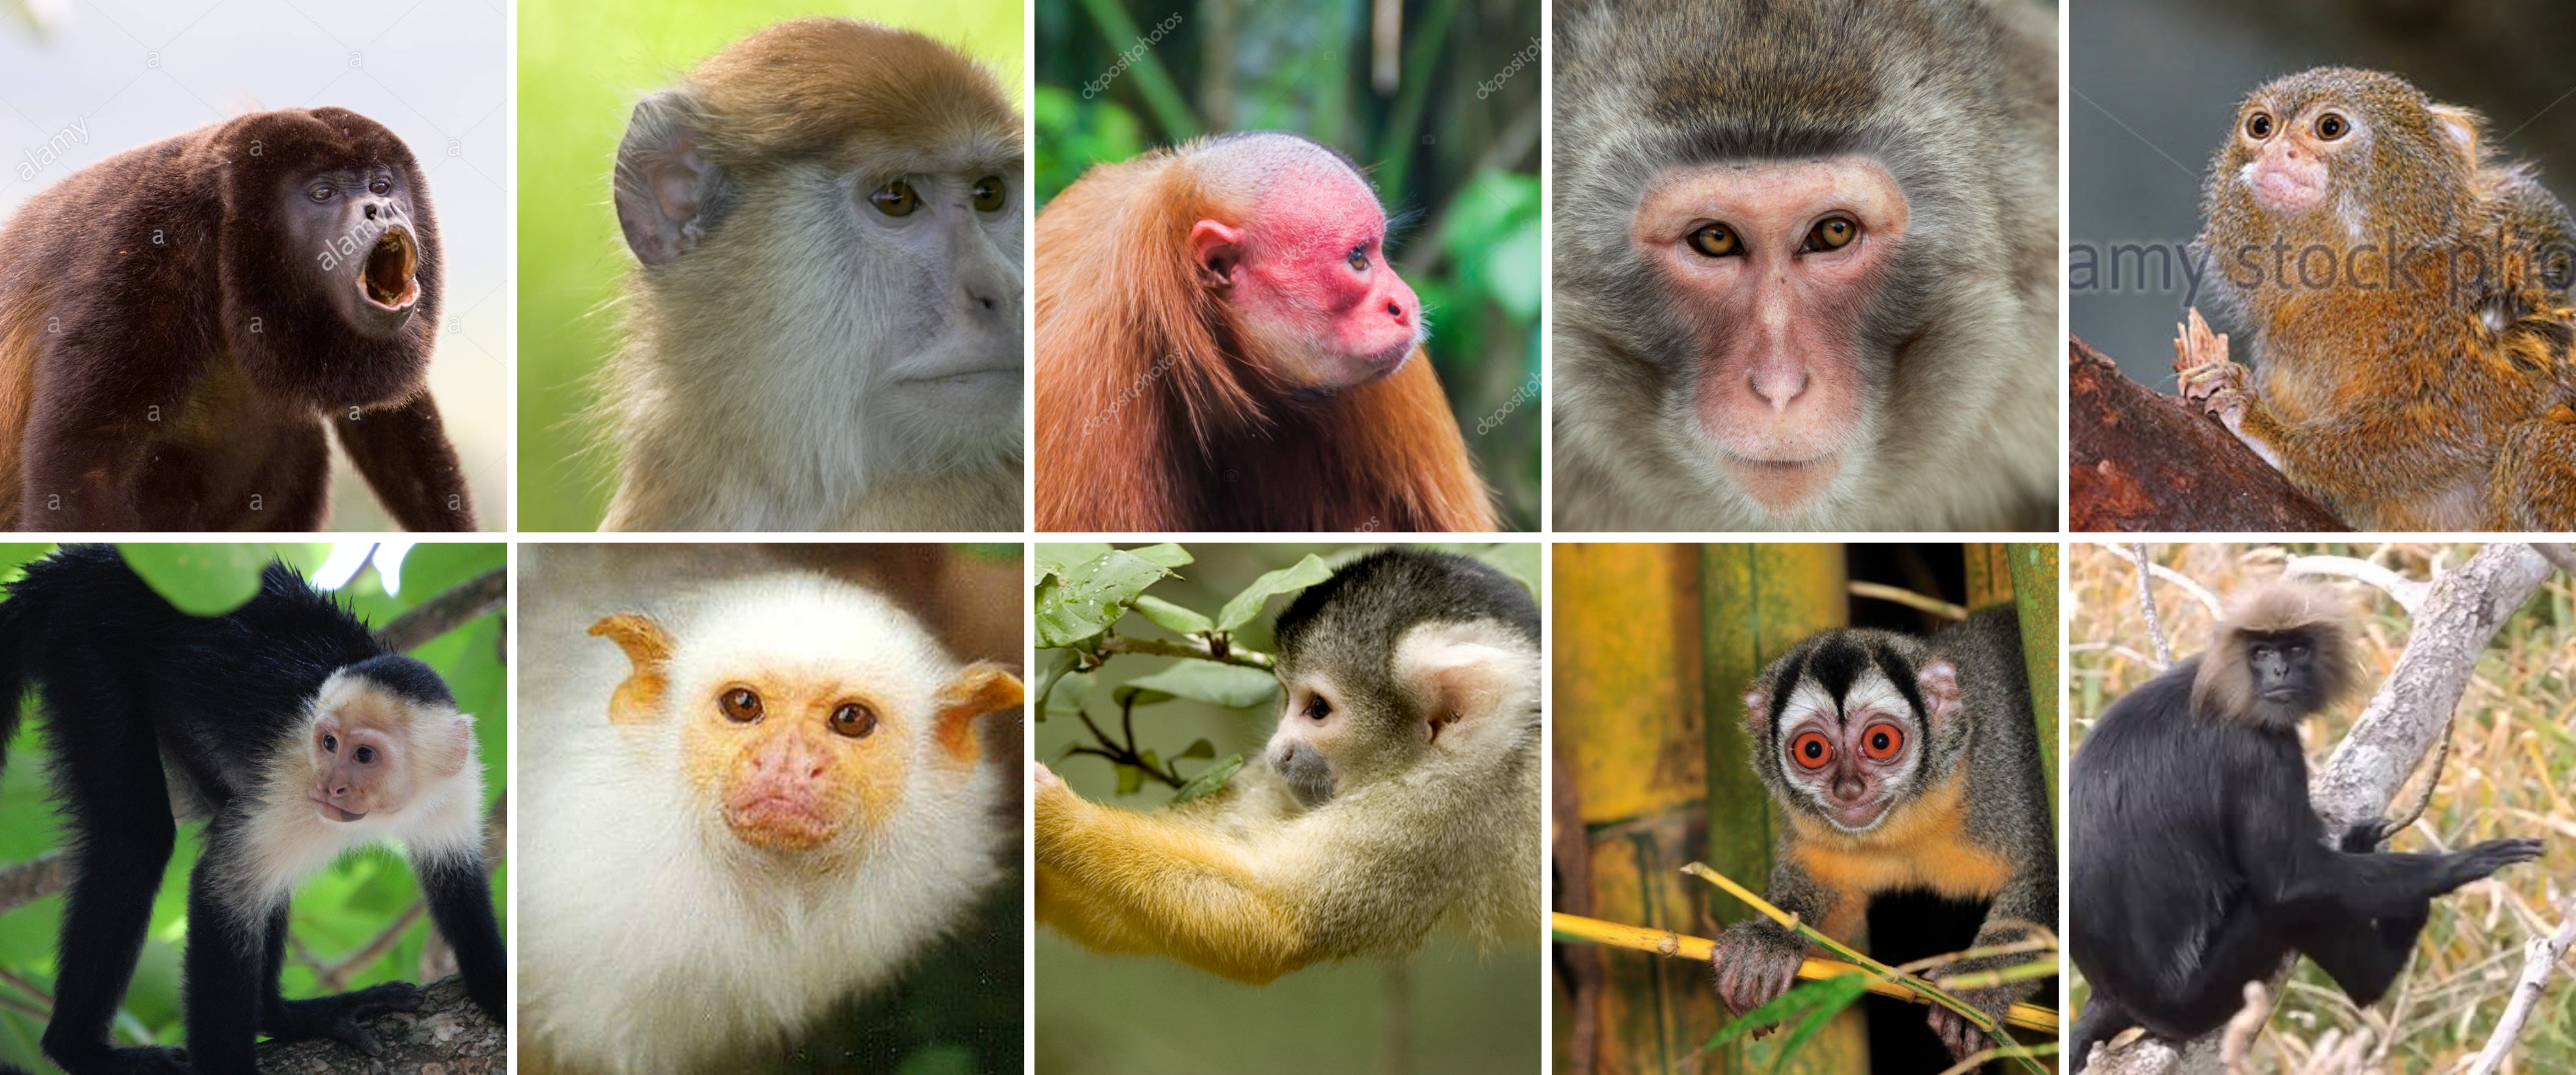
\includegraphics[scale=0.08]{img/2_monkey10-image.jpg}
\caption{Überblick über die verschiedenen Klassen des Monkey10 Datensatzes \cite{pawaraMonkey}.}
\label{fig:monkeyUeberblick}
\end{figure}

Der Pawara-Monkey10 Datensatz besteht aus insgesamt 1370 Bildern und ist mit 131 bis 152 Bildern je Klasse noch relativ gut ausbalanciert (s. Abb \ref{fig:Pawara-Monkey10Zusammensetzung}).\\

Im Gegensatz dazu ist der Datensatz Pawara-uMonkey10 weder in der Anzahl an Bildern pro Klasse noch in der Größe der Folds im Trainsplit ausbalanciert (s. Abb. \ref{fig:Pawara-uMonkey10Zusammensetzung}). 


\begin{figure}[H]
\begin{adjustbox}{width=1.4\textwidth, center}
\includesvg{img/2_pawara-monkey10_Zusammensetzung}
\end{adjustbox}
\caption{Aufteilung des Pawara-Monkey10 Datensatzes \cite{pawaraWebsiteDatensaetze} in Train- und Testsplits je Fold.}
\label{fig:Pawara-Monkey10Zusammensetzung}
\end{figure}
\begin{figure}[H]
\begin{adjustbox}{width=1.4\textwidth, center}
\includesvg{img/2_pawara-umonkey10_Zusammensetzung}
\end{adjustbox}
\caption{Aufteilung des unbalancierten Pawara-uMonkey10 Datensatzes \cite{pawaraWebsiteDatensaetze} in Train- und Testsplits je Fold.}
\label{fig:Pawara-uMonkey10Zusammensetzung}
\end{figure}





\subsection{SwedishLeaves}
\label{ch:methodik_SwedishLeaves}
Der SwedishLeaves Datensatz besteht aus Bildern von Blättern schwedischer Bäume, die zentriert auf einem weißen Hintergrund liegen (s. Abb. \ref{fig:swedishLeavesUeberblick}). Dadurch besitzen Bilder innerhalb einer Klasse eine hohe Ähnlichkeit.

\begin{figure}[H]
\centering
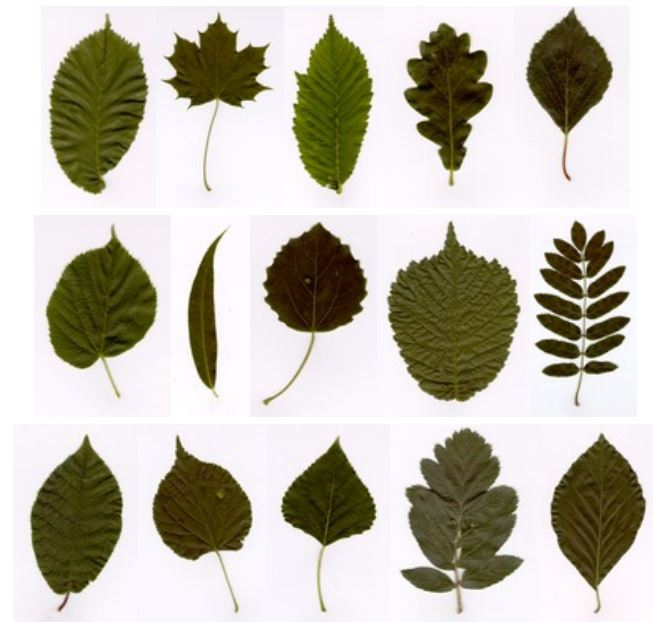
\includegraphics[scale=0.8]{img/2_swedishLeaves-image.jpg}
\caption{Überblick über die verschiedenen Klassen des SwedishLeaf Datensatzes \cite{pawaraMonkey}.}
\label{fig:swedishLeavesUeberblick}
\end{figure}

In den Experimenten von Pawara et al. \cite{pawaraPaper} wurde fünfmal ein Verhältnis von 1:2 für Trainings- und Testdaten aus den 75 Bildern pro Klasse gezogen (vgl. \cite{pawaraPaper} Kapitel 3.1.3), sodass im Testsplit doppelt so viele Bilder sind wie im Trainsplit.

Da hierbei offensichtlich Doppelungen zwischen den Folds entstehen und die verwendete Einteilung der Autorin des Papers \cite{pawaraPaper} nicht verfügbar ist, habe ich mich dafür entschieden die 75 Bilder pro Klasse in 3 Gruppen zu je 25 Bildern auf zu teilen und daraus 3 Folds mit einem Verhältnis von 1:2 für Trainings und Testdaten zu mischen. Dabei gelangt jedes Bild genau in einem Fold in den Trainsplit und in zwei Folds in den Testsplit. Es entsteht quasi eine 3-Fold Cross Validation mit vertauschtem Train- und Testsplit (s. Abb. \ref{fig:swedishLeavesZusammensetzung}).

Zusätzlich zu SwedishLeaves15 wurde mit drei weiteren Teilmengen des Datensatzes gearbeitet: SwedishLeaves10, SwedishLeaves5 und SwedishLeaves3.

\begin{figure}[H]
\begin{adjustbox}{width=1.4\textwidth, center}
\includesvg{img/2_swedishLeaves15_Zusammensetzung}
\end{adjustbox}
\caption{Aufteilung des SwedishLeaves15 Datensatzes \cite{swedishLeaves} in Train- und Testsplits je Fold.}
\label{fig:swedishLeavesZusammensetzung}
\end{figure}

\subsection{Tropic}
In dem Tropic Datensatz \cite{pawaraWebsiteDatensaetze} befinden sich 20 Klassen mit Bildern tropischer Pflanzen und deren Blättern, Blüten und Früchten (s. Abb. \ref{fig:tropicUeberblick}). Da unterschiedliche Teile der Pflanzen aus verschiedenen Blickwinkeln vor vielfältigen Hintergründen wie z.B. Erde, Himmel, Straßen oder Häusern fotografiert wurden ist die Klassifikation im Vergleich zum SwedishLeaves Datensatz \cite{swedishLeaves} (s. Kapitel \ref{ch:methodik_SwedishLeaves}) wesentlich anspruchsvoller.


\begin{figure}[H]
\centering
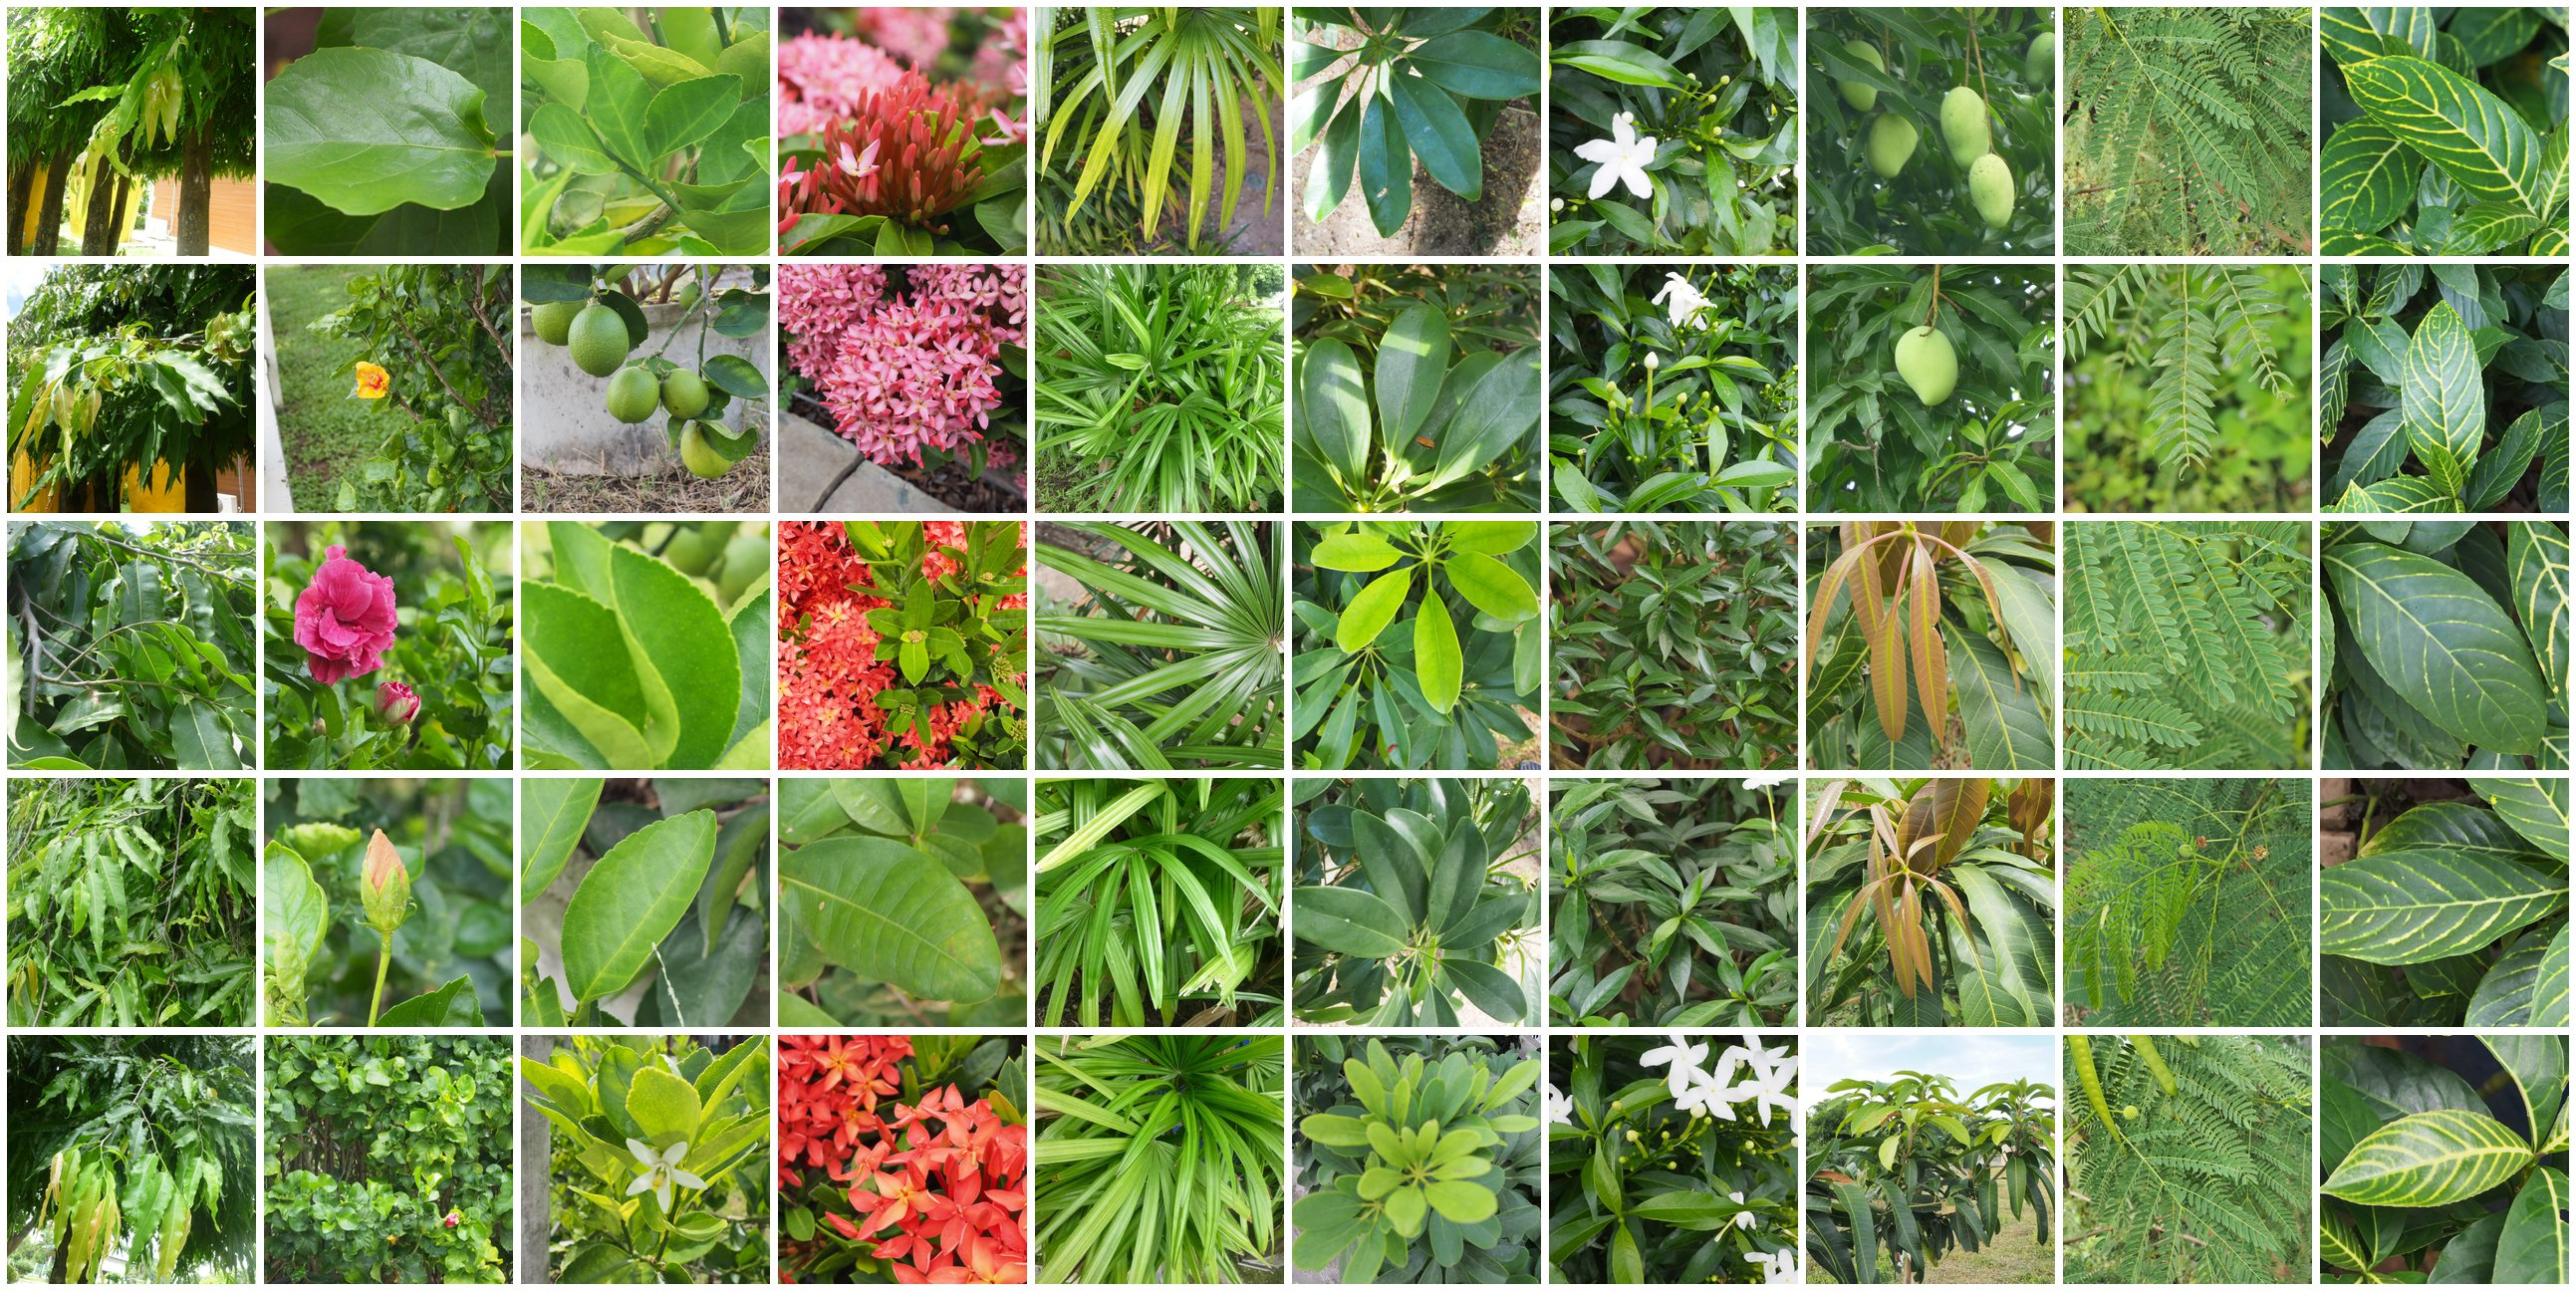
\includegraphics[scale=0.14]{img/2_tropic10-image.jpg}
\caption{Überblick über die verschiedenen Klassen des\\
Tropic Datensatzes \cite{pawaraTropic}.}
\label{fig:tropicUeberblick}
\end{figure}

Pro Klasse existieren 221-371 Bilder (s. Abb. \ref{fig:tropic20Zusammensetzung} und Abb. \ref{fig:pawaraTropic10Zusammensetzung}) in einer Auflösung von 250x250 Pixeln.

Es wurden Teilmengen von diesem Datensatz mit 20, 10, 5 und 3 Klassen zum Vergleich der beiden Klassifikationsschemata verwendet. Außerdem wurde die von Pawara et al. im Paper \cite{pawaraPaper} verwendete Einteilung in Folds \textit{Pawara-Tropic10} \cite{pawaraWebsiteDatensaetze} benutzt, bei der die 5-Fold Cross Validation aus fünfmaligem, zufälligem Ziehen eines Verhältnisses 70:30 für Trainings- und Testdaten besteht (s. Abb. \ref{fig:pawaraTropic10Zusammensetzung}).
Zusätzlich existiert noch ein Tropic52 Datensatz \cite{pawaraWebsiteDatensaetze} mit 52 Klassen, der aber weder im Paper von Pawara et al. \cite{pawaraPaper} noch in dieser Bachelorarbeit behandelt wird.

\begin{figure}[H]
\begin{adjustbox}{width=1.4\textwidth, center}
\includesvg{img/2_tropic20_Zusammensetzung}
\end{adjustbox}
\caption{Aufteilung des Tropic20 Datensatzes \cite{pawaraWebsiteDatensaetze} in Train- und Testsplits je Fold.}
\label{fig:tropic20Zusammensetzung}
\end{figure}
\begin{figure}[H]
\begin{adjustbox}{width=1.4\textwidth, center}
\includesvg{img/2_pawara-tropic10_Zusammensetzung}
\end{adjustbox}
\caption{Aufteilung des Pawara-Tropic10 Datensatzes \cite{pawaraWebsiteDatensaetze} in Train- und Testsplits je Fold.}
\label{fig:pawaraTropic10Zusammensetzung}
\end{figure}


\section{Trainingsparameter}
\label{ch:methodik_parameter}
Um zu untersuchen wie OvO und OvA im Vergleich zueinander in verschiedenen Situationen abschneiden, werden die folgenden Trainingsparameter für beide Klassifikationsschemata variiert.
Dadurch kann eine allgemeinere Aussage über die Vor- und Nachteile der OvO und OvA Klassifikation getroffen werden, da man durch die Variation der Trainingsparameter einen größeren Bereich an potentiellen Anwendungsfällen abdeckt.

Außerdem kann durch die verschiedenen Trainingsparameter analysiert werden, in welchen Situationen die OvO Klassifikation seine theoretischen Vorteile in der Praxis besonders gut ausnutzen kann und wann sich eine Implementation des OvO Klassifikationsschemas eher nicht lohnt.

\subsection{Frameworks}
Zu Beginn wurde das Training für diese Bachelorarbeit mit TensorFlow 2.4.1 \cite{tensorflow} durchgeführt. Jedoch wurde schnell deutlich, dass die Ergebnisse mit dieser Version von TensorFlow nicht den Erwartungen entsprechen und nicht mit den im Paper von Pawara et al. \cite{pawaraPaper} vorgestellten Ergebnissen übereinstimmen. Dabei sind die Abweichungen bei einigen Datensätzen und Kombinationen von Trainingsparametern deutlich größer als bei anderen (s. Kapitel \ref{ch:ergebnisse} und \ref{ch:diskussion}). \\

Die Autoren haben leider nicht angegeben, mit welcher Version von TensorFlow \cite{tensorflow} ihre Experimente durchgeführt wurden. Aber anhand des Veröffentlichungsdatums des Papers \cite{pawaraPaper} kann grob abgeschätzt werden, welche Version möglicherweise verwendet wurde.

Somit wurden zusätzlich die gleichen Experimente erneut mit der auf Palma II \cite{palma2} bereits vorinstallierten TensorFlow \cite{tensorflow} Version 1.13.1 durchgeführt.

Da zwischen diesen beiden Versionen von TensorFlow \cite{tensorflow} bereits erhebliche Diskrepanzen aufgetreten sind, wurden zum Schluss erneut die gleichen Experimente in PyTorch 1.9.0 \cite{pytorch} durchgeführt.
Damit soll sichergestellt werden, dass die Aussage über die Auswirkung der OvO oder OvA Klassifikation nicht nur auf bestimmte Versionen von TensorFlow \cite{tensorflow} zutrifft sondern möglichst allgemeingültig auf andere Machine-Learning Frameworks übertragen werden kann.

\todo{Implementation von Resnet und Inception vergleichen}

\subsection{Netztypen}
\label{ch:methodik_netze}
Für das Training werden die zwei beliebten Netzarchitekturen \textit{ResNet-50} und \textit{Inception V3} verwendet. Als Auflösung der Bilder für die Netze wurde bei \textit{ResNet-50} standardmäßig 224x224 Pixel und bei \textit{Inception V3} 299x299 Pixel verwendet. Größere oder kleinere Bilder in den Datensätzen wurden entsprechend skaliert.

Für das Netz \textit{Inception V3} hat die Autorin in dem auf Ihrer Webseite zur Verfügung gestellten Quellcode \cite{pawaraWebsiteCode} einige Änderungen an den letzten Schichten des Netzes vorgenommen. So wird beispielsweise eine zusätzliche \textit{BatchNormalization}-Schicht und eine \textit{Dropout}-Schicht eingefügt, die es in der Standardimplementierung von \textit{Inception V3} nicht gibt (s. Abb. \ref{fig:inceptionAenderungen}).

Die letzte Schicht, die \textit{Dense} oder \textit{Fully Connected} Schicht, wurde für OvO und OvA jeweils auf die entsprechende Anzahl an Klassifikatoren angepasst. Für die OvA Klassifikation hat das Netz genau so viele Ausgabewerte wie es Klassen gibt, für OvO gibt das Netz bei $k$ Klassen $\frac{k(k-1)}{2}$ Werte entsprechend des OvO Kodierungsschemas (s. Kapitel \ref{ch:methodik_kodierung}) aus.

\begin{figure}[H]

\begin{minipage}{.5\textwidth}
\begin{figure}[H]
\begin{adjustbox}{width=\textwidth, center}
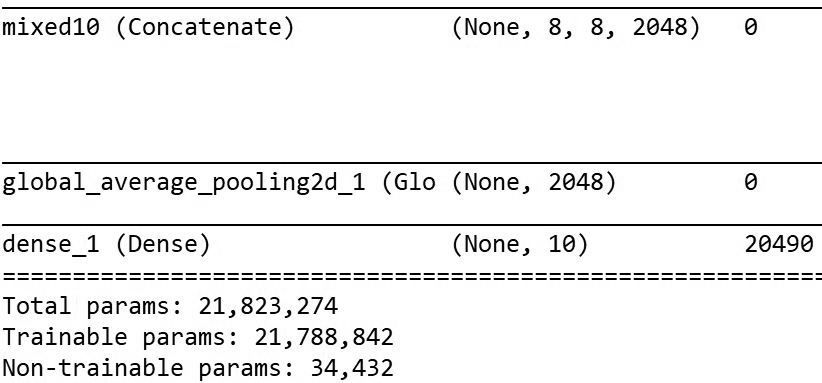
\includegraphics[scale=1]{img/3_inception-standard.jpg}
\end{adjustbox}
\end{figure}
\end{minipage}%
\begin{minipage}{.5\textwidth}
\begin{figure}[H]
\begin{adjustbox}{width=\textwidth, center}
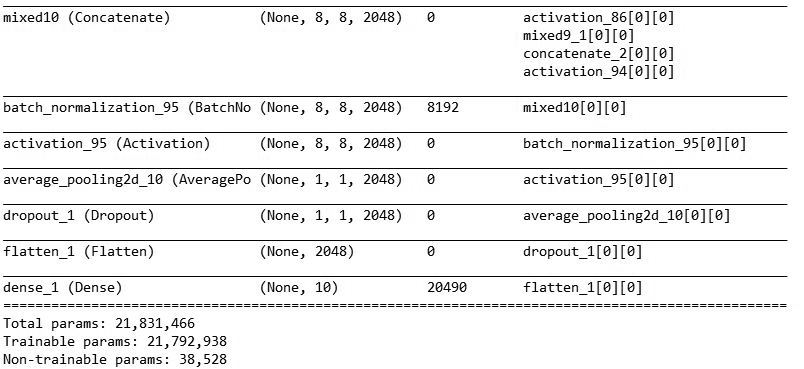
\includegraphics[scale=1]{img/3_inception-pawara.jpg}
\end{adjustbox}

\end{figure}
\end{minipage}
\caption{Standardmäßiger Aufbau des \textit{Inception V3} Netzes (links) und Änderungen an den letzten Schichten des \textit{Inception V3} Netzes von Pawara et al. \cite{pawaraWebsiteCode} (rechts).}
\label{fig:inceptionAenderungen}
\end{figure}


\subsection{Trainsize}

\todo{deterministische Datensatz-Splits}

\subsection{Klassenanzahl}

\subsection{vortrainierte Gewichte}
\todo{Epochen, Learningrate}


\section{Ausführung der Jobs auf Palma II}
\label{ch:methodik_palma}
\todo{Hardware auf Palma, Einteilung in Jobs, Logging, benutzte Grafikkarten, CPU Limits}



\chapter{Ergebnisse}
\label{ch:ergebnisse}

\todo{Alle Ergebnisse einfügen, Scatterplots für Acc und evtl. Dauer (normalisiert bezüglich Leistung der Grafikkarten)}
\todo{Confusion-Matrix für ein Beispiel raussuchen}
\todo{unspannende Sachen in den Anhang verschieben}
\todo{Trainingsverlauf exemplarisch plotten (Accuracy und Loss OvO vs OvA, evtl. für alle verschiedenen Frameworks)}
\todo{Probleme mit neuer TF Version, Github Issue}

\chapter{Diskussion}
\label{ch:diskussion}
\todo{schlechte Zahlen auf monkey (passt nicht zum Paper)}
\todo{generell die Zahlen mit denen aus dem Paper in Bezug setzen, besonders auf den Datensätzen die identisch sein sollten (mit Ausnahme der zufälligen Subsets)}
\todo{Ergebnisse diskutieren, vergleichen, (erste) Aussage treffen}

\section{OvO vs OvA}
\todo{OvO ist fast immer besser als OvA?}

\section{verschiedene Frameworks}
\todo{TF Versionen und Torch vergleichen (besonders swedishLeaves)}



\todo{Trainingsdauer-Plot erklären, num Workers bei torch höher, Optimierungen}
\todo{S vs F}
\todo{Probleme mit neuer TF Version, Github Issue}

\chapter{Fazit}
\label{ch:fazit}
Alles in allem konnten in dieser Arbeit die Ergebnisse von Pawara et al. \cite{pawaraPaper} bestätigt werden.\\
Durch die vielen Kombinationen an Parametern für das Training wurde der OvO und OvA Ansatz unter verschiedensten Bedingungen untersucht und miteinander verglichen.

Dabei ist die Verwendung eines OvO Klassifikationsschemas besonders bei Trainingsdurchläufen \textit{from Scratch}, also mit zufällig initialisierten Gewichten, und wenigen Trainingsbeispielen vielversprechend und kann sowohl zu einem stabileren Trainingsverlauf als auch zu besseren Ergebnissen beitragen.

Darüber hinaus gestaltet sich die Implementation eines OvO Klassifikationsschemas vergleichsweise einfach (vgl. Kapitel \ref{ch:methodik}). Somit ist es bei dem Training von tiefen neuronalen Netzen \textit{from Scratch} eindeutig ratsam, das OvO Klassifikationsschema anzuwenden bzw. zu untersuchen, ob der OvO Ansatz bei der konkreten Problemstellung von Vorteil ist. Besonders wenn das Training mit wenigen Trainingsdaten durchgeführt werden muss, bringt das OvO Klassifikationsschema in fast allen Fällen eine Verbesserung der Ergebnisse im Vergleich zu dem standardmäßig verwendeten OvA Ansatz (vgl. Kapitel \ref{ch:diskussionOvOvsOvA}) mit sich. Die Wahl des Klassifikationsschemas kann also als ein weiterer möglicher Hyperparameter für das Training tiefer neuronaler Netze verstanden werden.\\\\

Leider musste in dieser Arbeit aber auch festgestellt werden, dass die Wahl des Frameworks erheblichen Einfluss auf die Qualität der Ergebnisse haben kann. So schneidet TensorFlow 2.4.1 \cite{tensorflow} im Vergleich zu den anderen beiden Frameworks eher schlecht ab. Nur dort treten unerklärliche Ausreißer nach unten und sehr instabile Trainingsverläufe auf. Es wirkt so, als wäre TensorFlow \cite{tensorflow} von Version 1.13.1 zu Version 2.4.1 zumindest bei den in dieser Arbeit durchgeführten Experimenten tatsächlich schlechter geworden.\\
PyTorch \cite{pytorch} hingegen scheint eine sehr gute Wahl zu sein, da die Ergebnisse auf einem vergleichbar guten Niveau wie bei TensorFlow 1.13.1 \cite{tensorflow} liegen, während die Trainingsdauer bedingt durch die bessere Auslastung der Grafikkarte größtenteils wesentlich kürzer ist als die von TensorFlow \cite{tensorflow} (vgl. Kapitel \ref{ch:diskussionFrameworks}).\\\\

\newpage

Weitere spannende Untersuchungen für die Zukunft könnten sich ergeben, wenn der OvO Ansatz auf komplett anderen Datensätzen untersucht wird. In dieser Arbeit, wie auch im Paper von Pawara et al. \cite{pawaraPaper}, wurden größtenteils Datensätze mit Bildern aus der Natur wie z.B. Bilder von Blättern, Früchten und Affen verwendet. Außerdem wäre es interessant zu untersuchen, ab welcher Klassenanzahl der Mehraufwand für das Training so stark angewachsen ist, dass der OvO Ansatz sich in dieser Form nicht mehr als praktikabel erweist.\\\\

Darüber hinaus kann an den in dieser Arbeit und im Paper von Pawara et al. \cite{pawaraPaper} verwendeten Hyperparametern gearbeitet werden. So zeigt sich besonders am Verlauf des Trainings (vgl. Abb. \ref{fig:TrainingsverlaufA}, \ref{fig:TrainingsverlaufB} und \ref{fig:TrainingsverlaufC}), dass immer in den Epochen nach einer Anpassung der Learning-Rate eine starke Veränderung sowohl bei den Loss- als auch Accuracy-Werten hervorgerufen wird. Eventuell wäre es ein guter Ansatz die Learning-Rate nicht sprunghaft alle 50 Epochen zu verringern, sondern sie während des Trainings kontinuierlich zu senken. Außerdem könnte die initiale Learning-Rate variiert werden, da die größten Fortschritte bei dem Training meistens nicht innerhalb der ersten 50 Epochen stattfinden (vgl. Kapitel \ref{ch:Beispiele}).\\\\

Eine weitere Möglichkeit für zukünftige Untersuchungen wäre es, wie Pawara et al. auch schon vorgeschlagen haben (vgl. \cite{pawaraPaper} Kapitel 6 Conclusion), bei Finetune Experimenten für faire Bedingungen zwischen den beiden Klassifikationsschemata zu sorgen, indem die auf ImageNet \cite{imagenet} vor-trainierten Gewichte mit dem jeweils passenden Klassifikationsschema erzeugt werden, sodass Finetuning Experimente mit dem OvO Ansatz auch vor-trainierte initiale Gewichte bekommen, die mit dem OvO Klassifikationsschema vor-trainiert wurden.


% Literaturverzeichnis
\bibliographystyle{unsrtdin}
\bibliography{Quellen}

% Anhang
% Platz vor Chapter-Überschrift verringern (damit auch auf die erste Seite 2 Tabellen untereinander passen)
\makeatletter
\let\savedchap\@makechapterhead
\def\@makechapterhead{\vspace*{-2cm}\savedchap}
\makeatletter
% Seitenränder verringern (unten und oben)
\newgeometry{top=0.5cm, bottom=0.5cm}


\chapter{Tabellen mit Ergebnissen}
\label{ch:Anhang_Tabellen}
\section{Tensorflow 1.13.1}

\subsection{Resnet Scratch}
\begin{figure}[H]
\resizebox{\textwidth}{!}{
\begin{tabular}{|c|c|c|}
\multicolumn{3}{c}{agrilplant3} \\
\hline
\hline
\scriptsize{Train Prozent} & OvO & OvA \\
\hline 10 & 78.67 \plm 1.45 & 77.67 \plm 2.84\\
20 & 84.44 \plm 1.42 & 85.00 \plm 4.04\\
50 & 96.00 \plm 1.86 & 94.22 \plm 2.17\\
80 & 97.00 \plm 1.01 & 96.67 \plm 0.88\\
100 & 98.33 \plm 0.68 & 97.89 \plm 0.61\\
\hline 
\end{tabular}

\begin{tabular}{|c|c|}
\multicolumn{2}{c}{agrilplant5} \\
\hline
\hline
OvO & OvA \\
\hline 75.93 \plm 2.20 & 74.13 \plm 4.17\\
87.40 \plm 3.72 & 85.40 \plm 4.41\\
96.80 \plm 1.07 & 95.60 \plm 1.89\\
97.67 \plm 0.97 & 97.60 \plm 0.89\\
98.27 \plm 0.55 & 97.73 \plm 0.95\\
\hline 
\end{tabular}

\begin{tabular}{|c|c|}
\multicolumn{2}{c}{agrilplant10} \\
\hline
\hline
OvO & OvA \\
\hline 74.37 \plm 3.58 & 69.93 \plm 5.32\\
84.80 \plm 2.25 & 83.53 \plm 2.54\\
92.47 \plm 1.18 & 92.47 \plm 0.36\\
95.33 \plm 0.86 & 95.33 \plm 0.67\\
96.03 \plm 0.62 & 95.77 \plm 0.61\\
\hline 
\end{tabular}
}%
\vspace{2mm}
\resizebox{\textwidth}{!}{
\begin{tabular}{|c|c|c|}
\multicolumn{3}{c}{tropic3} \\
\hline
\hline
\scriptsize{Train Prozent} & OvO & OvA \\
\hline 10 & 88.96 \plm 2.78 & 87.75 \plm 4.49\\
20 & 92.72 \plm 1.48 & 91.51 \plm 1.28\\
50 & 98.18 \plm 1.83 & 97.69 \plm 1.32\\
80 & 98.06 \plm 0.79 & 97.93 \plm 1.40\\
100 & 99.03 \plm 0.92 & 98.91 \plm 0.90\\
\hline 
\end{tabular}

\begin{tabular}{|c|c|}
\multicolumn{2}{c}{tropic5} \\
\hline
\hline
OvO & OvA \\
\hline 78.72 \plm 2.04 & 76.90 \plm 3.63\\
89.03 \plm 3.15 & 86.86 \plm 3.51\\
96.08 \plm 1.96 & 96.59 \plm 1.04\\
97.90 \plm 1.41 & 98.77 \plm 1.16\\
99.13 \plm 0.41 & 98.62 \plm 0.65\\
\hline 
\end{tabular}

\begin{tabular}{|c|c|}
\multicolumn{2}{c}{tropic10} \\
\hline
\hline
OvO & OvA \\
\hline 76.48 \plm 1.08 & 67.67 \plm 4.78\\
87.51 \plm 1.41 & 82.66 \plm 1.80\\
95.15 \plm 0.38 & 94.25 \plm 1.32\\
97.14 \plm 0.56 & 97.73 \plm 0.33\\
98.08 \plm 0.59 & 97.77 \plm 0.75\\
\hline 
\end{tabular}

\begin{tabular}{|c|c|}
\multicolumn{2}{c}{tropic20} \\
\hline
\hline
OvO & OvA \\
\hline 73.50 \plm 1.51 & 70.93 \plm 1.82\\
84.55 \plm 2.16 & 81.99 \plm 2.54\\
93.16 \plm 2.02 & 94.05 \plm 1.61\\
96.21 \plm 0.80 & 96.30 \plm 0.75\\
96.74 \plm 0.93 & 97.78 \plm 0.59\\
\hline 
\end{tabular}
}%
\vspace{2mm}
\resizebox{\textwidth}{!}{
\begin{tabular}{|c|c|c|}
\multicolumn{3}{c}{swedishLeaves3folds3} \\
\hline
\hline
\scriptsize{Train Prozent} & OvO & OvA \\
\hline 10 & 58.67 \plm 7.33 & 55.78 \plm 7.78\\
20 & 67.11 \plm 6.74 & 69.11 \plm 2.69\\
50 & 85.56 \plm 1.02 & 87.33 \plm 1.76\\
80 & 91.56 \plm 1.02 & 90.89 \plm 1.92\\
100 & 94.00 \plm 1.33 & 94.22 \plm 2.52\\
\hline 
\end{tabular}

\begin{tabular}{|c|c|}
\multicolumn{2}{c}{swedishLeaves3folds5} \\
\hline
\hline
OvO & OvA \\
\hline 58.53 \plm 11.21 & 44.13 \plm 9.75\\
84.40 \plm 2.62 & 82.27 \plm 5.83\\
93.33 \plm 1.29 & 91.73 \plm 1.67\\
95.73 \plm 2.81 & 94.80 \plm 1.06\\
97.07 \plm 0.46 & 95.47 \plm 0.83\\
\hline 
\end{tabular}

\begin{tabular}{|c|c|}
\multicolumn{2}{c}{swedishLeaves3folds10} \\
\hline
\hline
OvO & OvA \\
\hline 76.93 \plm 4.32 & 78.13 \plm 4.21\\
87.40 \plm 2.08 & 89.00 \plm 1.11\\
93.13 \plm 1.45 & 92.07 \plm 2.50\\
95.07 \plm 1.81 & 94.00 \plm 1.97\\
96.80 \plm 0.69 & 96.53 \plm 0.90\\
\hline 
\end{tabular}

\begin{tabular}{|c|c|}
\multicolumn{2}{c}{swedishLeaves3folds15} \\
\hline
\hline
OvO & OvA \\
\hline 65.82 \plm 11.74 & 71.20 \plm 4.80\\
91.60 \plm 1.16 & 88.40 \plm 3.20\\
93.16 \plm 1.44 & 93.38 \plm 1.16\\
96.84 \plm 0.20 & 94.80 \plm 3.84\\
97.11 \plm 0.15 & 96.84 \plm 0.73\\
\hline 
\end{tabular}
}%
\vspace{2mm}
\resizebox{\textwidth}{!}{
\begin{tabular}{|c|c|c|}
\multicolumn{3}{c}{pawara-tropic10} \\
\hline
\hline
\scriptsize{Train Prozent} & OvO & OvA \\
\hline 10 & 69.74 \plm 3.69 & 64.42 \plm 3.61\\
20 & 83.54 \plm 1.48 & 78.06 \plm 0.96\\
50 & 93.66 \plm 1.81 & 92.90 \plm 1.17\\
80 & 96.66 \plm 0.68 & 97.08 \plm 0.76\\
100 & 97.94 \plm 0.55 & 97.81 \plm 0.60\\
\hline 
\end{tabular}

\begin{tabular}{|c|c|}
\multicolumn{2}{c}{pawara-monkey10} \\
\hline
\hline
OvO & OvA \\
\hline 47.81 \plm 2.62 & 42.57 \plm 2.77\\
59.33 \plm 2.78 & 57.29 \plm 2.62\\
73.38 \plm 8.29 & 71.46 \plm 3.46\\
86.79 \plm 1.53 & 86.42 \plm 1.58\\
89.05 \plm 1.18 & 89.12 \plm 1.85\\
\hline 
\end{tabular}

\begin{tabular}{|c|c|}
\multicolumn{2}{c}{pawara-umonkey10} \\
\hline
\hline
OvO & OvA \\
\hline 31.97 \plm 1.63 & 32.56 \plm 3.61\\
43.64 \plm 3.75 & 38.83 \plm 1.76\\
60.01 \plm 3.48 & 56.72 \plm 4.37\\
67.67 \plm 0.96 & 67.01 \plm 1.96\\
69.65 \plm 5.30 & 68.47 \plm 3.21\\
\hline 
\end{tabular}

\begin{tabular}{|c|c|}
\multicolumn{2}{c}{cifar10} \\
\hline
\hline
OvO & OvA \\
\hline 76.50 \plm 1.08 & 79.09 \plm 1.44\\
83.91 \plm 0.86 & 85.41 \plm 0.67\\
90.16 \plm 0.50 & 90.68 \plm 0.47\\
92.17 \plm 0.54 & 92.70 \plm 0.66\\
92.84 \plm 0.93 & 93.87 \plm 0.18\\
\hline 
\end{tabular}
}%

\end{figure}

\subsection{Resnet Finetune}
\begin{figure}[H]
\resizebox{\textwidth}{!}{
\begin{tabular}{|c|c|c|}
\multicolumn{3}{c}{agrilplant3} \\
\hline
\hline
\scriptsize{Train Prozent} & OvO & OvA \\
\hline 10 & 99.00 \plm 0.61 & 99.22 \plm 0.63\\
20 & 99.67 \plm 0.50 & 99.44 \plm 0.56\\
50 & 99.89 \plm 0.25 & 99.56 \plm 0.25\\
80 & 100.00 \plm 0.00 & 99.89 \plm 0.25\\
100 & 100.00 \plm 0.00 & 100.00 \plm 0.00\\
\hline 
\end{tabular}

\begin{tabular}{|c|c|}
\multicolumn{2}{c}{agrilplant5} \\
\hline
\hline
OvO & OvA \\
\hline 95.40 \plm 1.36 & 94.73 \plm 1.55\\
98.33 \plm 0.91 & 96.80 \plm 0.77\\
99.13 \plm 0.38 & 99.27 \plm 0.76\\
99.60 \plm 0.28 & 99.73 \plm 0.28\\
99.40 \plm 0.55 & 99.87 \plm 0.18\\
\hline 
\end{tabular}

\begin{tabular}{|c|c|}
\multicolumn{2}{c}{agrilplant10} \\
\hline
\hline
OvO & OvA \\
\hline 92.03 \plm 1.28 & 92.67 \plm 0.73\\
95.23 \plm 0.78 & 95.77 \plm 0.84\\
96.90 \plm 0.45 & 97.70 \plm 0.77\\
97.87 \plm 0.41 & 98.67 \plm 0.51\\
98.07 \plm 0.42 & 98.67 \plm 0.42\\
\hline 
\end{tabular}
}%
\vspace{2mm}
\resizebox{\textwidth}{!}{
\begin{tabular}{|c|c|c|}
\multicolumn{3}{c}{tropic3} \\
\hline
\hline
\scriptsize{Train Prozent} & OvO & OvA \\
\hline 10 & 98.30 \plm 0.79 & 96.60 \plm 1.85\\
20 & 99.51 \plm 0.27 & 99.27 \plm 0.27\\
50 & 99.76 \plm 0.33 & 99.39 \plm 0.61\\
80 & 99.27 \plm 0.27 & 100.00 \plm 0.00\\
100 & 99.88 \plm 0.27 & 99.76 \plm 0.54\\
\hline 
\end{tabular}

\begin{tabular}{|c|c|}
\multicolumn{2}{c}{tropic5} \\
\hline
\hline
OvO & OvA \\
\hline 96.37 \plm 1.03 & 95.72 \plm 1.10\\
98.76 \plm 1.14 & 98.62 \plm 0.83\\
99.56 \plm 0.30 & 99.35 \plm 0.16\\
99.56 \plm 0.16 & 99.85 \plm 0.20\\
99.71 \plm 0.30 & 99.78 \plm 0.20\\
\hline 
\end{tabular}

\begin{tabular}{|c|c|}
\multicolumn{2}{c}{tropic10} \\
\hline
\hline
OvO & OvA \\
\hline 92.92 \plm 1.08 & 94.87 \plm 0.82\\
96.48 \plm 0.91 & 97.69 \plm 0.45\\
98.86 \plm 0.42 & 99.45 \plm 0.40\\
98.98 \plm 0.32 & 99.61 \plm 0.48\\
99.41 \plm 0.37 & 99.73 \plm 0.30\\
\hline 
\end{tabular}

\begin{tabular}{|c|c|}
\multicolumn{2}{c}{tropic20} \\
\hline
\hline
OvO & OvA \\
\hline 91.36 \plm 0.81 & 94.24 \plm 1.13\\
95.81 \plm 0.63 & 97.48 \plm 0.50\\
97.99 \plm 0.53 & 98.82 \plm 0.49\\
98.90 \plm 0.13 & 99.34 \plm 0.24\\
99.05 \plm 0.35 & 99.66 \plm 0.11\\
\hline 
\end{tabular}
}%
\vspace{2mm}
\resizebox{\textwidth}{!}{
\begin{tabular}{|c|c|c|}
\multicolumn{3}{c}{swedishLeaves3folds3} \\
\hline
\hline
\scriptsize{Train Prozent} & OvO & OvA \\
\hline 10 & 84.22 \plm 6.58 & 86.00 \plm 1.76\\
20 & 92.44 \plm 3.91 & 91.11 \plm 2.78\\
50 & 95.33 \plm 3.53 & 94.67 \plm 4.81\\
80 & 99.78 \plm 0.38 & 97.33 \plm 1.33\\
100 & 98.44 \plm 0.38 & 98.67 \plm 0.67\\
\hline 
\end{tabular}

\begin{tabular}{|c|c|}
\multicolumn{2}{c}{swedishLeaves3folds5} \\
\hline
\hline
OvO & OvA \\
\hline 93.47 \plm 0.61 & 92.53 \plm 1.51\\
96.13 \plm 3.45 & 96.93 \plm 2.95\\
99.07 \plm 0.23 & 97.60 \plm 2.12\\
99.20 \plm 0.80 & 99.73 \plm 0.23\\
99.60 \plm 0.40 & 99.73 \plm 0.23\\
\hline 
\end{tabular}

\begin{tabular}{|c|c|}
\multicolumn{2}{c}{swedishLeaves3folds10} \\
\hline
\hline
OvO & OvA \\
\hline 94.20 \plm 2.46 & 93.13 \plm 1.70\\
97.73 \plm 0.23 & 96.40 \plm 0.20\\
97.13 \plm 1.70 & 97.13 \plm 2.39\\
99.20 \plm 0.72 & 99.47 \plm 0.50\\
99.73 \plm 0.31 & 99.80 \plm 0.20\\
\hline 
\end{tabular}

\begin{tabular}{|c|c|}
\multicolumn{2}{c}{swedishLeaves3folds15} \\
\hline
\hline
OvO & OvA \\
\hline 96.98 \plm 0.73 & 95.64 \plm 1.26\\
98.40 \plm 0.46 & 97.87 \plm 0.81\\
99.16 \plm 0.60 & 98.89 \plm 0.28\\
99.56 \plm 0.28 & 99.69 \plm 0.20\\
99.56 \plm 0.31 & 99.82 \plm 0.20\\
\hline 
\end{tabular}
}%
\vspace{2mm}
\resizebox{\textwidth}{!}{
\begin{tabular}{|c|c|c|}
\multicolumn{3}{c}{pawara-tropic10} \\
\hline
\hline
\scriptsize{Train Prozent} & OvO & OvA \\
\hline 10 & 93.69 \plm 1.49 & 94.60 \plm 1.04\\
20 & 95.43 \plm 1.51 & 97.08 \plm 1.06\\
50 & 98.38 \plm 0.51 & 99.43 \plm 0.20\\
80 & 99.09 \plm 0.28 & 99.63 \plm 0.11\\
100 & 99.32 \plm 0.34 & 99.74 \plm 0.21\\
\hline 
\end{tabular}

\begin{tabular}{|c|c|}
\multicolumn{2}{c}{pawara-monkey10} \\
\hline
\hline
OvO & OvA \\
\hline 89.41 \plm 1.93 & 90.95 \plm 1.21\\
93.43 \plm 2.07 & 93.36 \plm 1.55\\
95.33 \plm 1.43 & 95.47 \plm 1.12\\
96.93 \plm 0.62 & 97.67 \plm 1.22\\
97.30 \plm 0.98 & 97.66 \plm 0.41\\
\hline 
\end{tabular}

\begin{tabular}{|c|c|}
\multicolumn{2}{c}{pawara-umonkey10} \\
\hline
\hline
OvO & OvA \\
\hline 73.80 \plm 3.01 & 70.31 \plm 3.36\\
84.38 \plm 1.97 & 81.24 \plm 2.34\\
90.58 \plm 1.56 & 88.32 \plm 2.03\\
91.09 \plm 2.09 & 91.15 \plm 2.40\\
93.28 \plm 0.45 & 91.75 \plm 2.04\\
\hline 
\end{tabular}
}%

\end{figure}

\newpage

\subsection{Inception Scratch}
\begin{figure}[H]
\resizebox{\textwidth}{!}{
\begin{tabular}{|c|c|c|}
\multicolumn{3}{c}{agrilplant3} \\
\hline
\hline
\scriptsize{Train Prozent} & OvO & OvA \\
\hline 10 & 80.44 \plm 2.06 & 82.78 \plm 4.46\\
20 & 89.11 \plm 1.34 & 87.89 \plm 1.90\\
50 & 96.89 \plm 1.01 & 97.67 \plm 0.72\\
80 & 98.33 \plm 0.88 & 98.33 \plm 0.79\\
100 & 98.11 \plm 1.15 & 98.44 \plm 0.25\\
\hline 
\end{tabular}

\begin{tabular}{|c|c|}
\multicolumn{2}{c}{agrilplant5} \\
\hline
\hline
OvO & OvA \\
\hline 82.47 \plm 1.79 & 80.73 \plm 2.62\\
90.20 \plm 1.28 & 88.73 \plm 3.95\\
97.33 \plm 0.53 & 97.53 \plm 0.96\\
98.47 \plm 0.45 & 98.20 \plm 0.65\\
98.87 \plm 0.77 & 98.93 \plm 0.55\\
\hline 
\end{tabular}

\begin{tabular}{|c|c|}
\multicolumn{2}{c}{agrilplant10} \\
\hline
\hline
OvO & OvA \\
\hline 78.60 \plm 2.68 & 74.47 \plm 2.88\\
87.43 \plm 1.64 & 86.90 \plm 1.72\\
94.07 \plm 0.56 & 94.07 \plm 0.56\\
96.40 \plm 0.71 & 96.07 \plm 0.49\\
96.47 \plm 0.72 & 97.23 \plm 0.52\\
\hline 
\end{tabular}
}%
\vspace{2mm}
\resizebox{\textwidth}{!}{
\begin{tabular}{|c|c|c|}
\multicolumn{3}{c}{tropic3} \\
\hline
\hline
\scriptsize{Train Prozent} & OvO & OvA \\
\hline 10 & 88.47 \plm 2.90 & 88.11 \plm 4.46\\
20 & 93.20 \plm 2.52 & 92.35 \plm 1.52\\
50 & 97.57 \plm 0.96 & 97.45 \plm 0.80\\
80 & 98.18 \plm 1.13 & 98.30 \plm 0.79\\
100 & 98.79 \plm 0.43 & 98.42 \plm 0.93\\
\hline 
\end{tabular}

\begin{tabular}{|c|c|}
\multicolumn{2}{c}{tropic5} \\
\hline
\hline
OvO & OvA \\
\hline 79.16 \plm 2.78 & 77.85 \plm 3.15\\
91.14 \plm 2.87 & 87.95 \plm 2.41\\
97.24 \plm 1.24 & 96.95 \plm 0.91\\
99.06 \plm 0.55 & 98.40 \plm 0.48\\
99.27 \plm 0.57 & 98.48 \plm 1.04\\
\hline 
\end{tabular}

\begin{tabular}{|c|c|}
\multicolumn{2}{c}{tropic10} \\
\hline
\hline
OvO & OvA \\
\hline 78.75 \plm 1.34 & 72.33 \plm 1.55\\
88.06 \plm 1.91 & 84.11 \plm 1.66\\
97.22 \plm 0.81 & 95.54 \plm 1.48\\
98.75 \plm 0.33 & 98.12 \plm 0.78\\
98.98 \plm 0.38 & 98.51 \plm 0.26\\
\hline 
\end{tabular}

\begin{tabular}{|c|c|}
\multicolumn{2}{c}{tropic20} \\
\hline
\hline
OvO & OvA \\
\hline 74.43 \plm 1.37 & 69.64 \plm 1.68\\
86.05 \plm 1.00 & 82.34 \plm 1.31\\
96.11 \plm 0.79 & 94.41 \plm 1.02\\
97.52 \plm 0.46 & 97.61 \plm 0.68\\
98.71 \plm 0.36 & 98.58 \plm 0.07\\
\hline 
\end{tabular}
}%
\vspace{2mm}
\resizebox{\textwidth}{!}{
\begin{tabular}{|c|c|c|}
\multicolumn{3}{c}{swedishLeaves3folds3} \\
\hline
\hline
\scriptsize{Train Prozent} & OvO & OvA \\
\hline 10 & 69.33 \plm 7.57 & 61.78 \plm 9.71\\
20 & 67.33 \plm 15.01 & 71.78 \plm 3.15\\
50 & 87.78 \plm 2.78 & 85.11 \plm 1.02\\
80 & 94.89 \plm 1.02 & 93.33 \plm 1.15\\
100 & 94.67 \plm 1.76 & 93.33 \plm 2.40\\
\hline 
\end{tabular}

\begin{tabular}{|c|c|}
\multicolumn{2}{c}{swedishLeaves3folds5} \\
\hline
\hline
OvO & OvA \\
\hline 66.27 \plm 2.84 & 64.27 \plm 8.26\\
88.40 \plm 1.39 & 85.60 \plm 3.17\\
93.20 \plm 3.12 & 92.00 \plm 1.06\\
95.87 \plm 1.01 & 94.13 \plm 0.61\\
98.80 \plm 0.69 & 96.13 \plm 0.92\\
\hline 
\end{tabular}

\begin{tabular}{|c|c|}
\multicolumn{2}{c}{swedishLeaves3folds10} \\
\hline
\hline
OvO & OvA \\
\hline 82.47 \plm 5.75 & 79.67 \plm 4.96\\
90.27 \plm 2.80 & 90.53 \plm 1.14\\
94.07 \plm 0.83 & 91.33 \plm 0.83\\
97.00 \plm 0.40 & 96.67 \plm 0.12\\
97.53 \plm 1.10 & 97.33 \plm 0.42\\
\hline 
\end{tabular}

\begin{tabular}{|c|c|}
\multicolumn{2}{c}{swedishLeaves3folds15} \\
\hline
\hline
OvO & OvA \\
\hline 83.64 \plm 3.81 & 79.96 \plm 2.65\\
92.09 \plm 3.35 & 88.80 \plm 1.67\\
94.27 \plm 0.61 & 92.93 \plm 1.62\\
98.09 \plm 0.38 & 98.09 \plm 0.96\\
98.13 \plm 0.48 & 98.13 \plm 0.13\\
\hline 
\end{tabular}
}%
\vspace{2mm}
\resizebox{\textwidth}{!}{
\begin{tabular}{|c|c|c|}
\multicolumn{3}{c}{pawara-tropic10} \\
\hline
\hline
\scriptsize{Train Prozent} & OvO & OvA \\
\hline 10 & 73.52 \plm 2.98 & 67.28 \plm 2.98\\
20 & 87.06 \plm 2.42 & 81.40 \plm 1.60\\
50 & 96.61 \plm 0.64 & 94.42 \plm 1.47\\
80 & 98.51 \plm 0.60 & 97.37 \plm 0.77\\
100 & 98.72 \plm 0.14 & 98.04 \plm 0.51\\
\hline 
\end{tabular}

\begin{tabular}{|c|c|}
\multicolumn{2}{c}{pawara-monkey10} \\
\hline
\hline
OvO & OvA \\
\hline 52.34 \plm 1.86 & 45.70 \plm 3.21\\
66.56 \plm 4.18 & 61.10 \plm 4.23\\
78.75 \plm 5.41 & 78.54 \plm 1.99\\
90.08 \plm 2.52 & 89.71 \plm 1.81\\
91.90 \plm 1.94 & 91.89 \plm 2.00\\
\hline 
\end{tabular}

\begin{tabular}{|c|c|}
\multicolumn{2}{c}{pawara-umonkey10} \\
\hline
\hline
OvO & OvA \\
\hline 37.51 \plm 3.27 & 34.73 \plm 3.44\\
46.87 \plm 4.88 & 45.47 \plm 5.71\\
61.47 \plm 6.48 & 60.50 \plm 6.18\\
71.97 \plm 2.76 & 68.25 \plm 1.79\\
75.83 \plm 1.95 & 72.19 \plm 1.53\\
\hline 
\end{tabular}
}%

\end{figure}
\subsection{Inception Finetune}
\begin{figure}[H]
\resizebox{\textwidth}{!}{
\begin{tabular}{|c|c|c|}
\multicolumn{3}{c}{agrilplant3} \\
\hline
\hline
\scriptsize{Train Prozent} & OvO & OvA \\
\hline 10 & 99.44 \plm 0.39 & 99.33 \plm 0.46\\
20 & 99.67 \plm 0.50 & 99.67 \plm 0.30\\
50 & 99.89 \plm 0.25 & 99.78 \plm 0.30\\
80 & 99.89 \plm 0.25 & 99.78 \plm 0.30\\
100 & 100.00 \plm 0.00 & 100.00 \plm 0.00\\
\hline 
\end{tabular}

\begin{tabular}{|c|c|}
\multicolumn{2}{c}{agrilplant5} \\
\hline
\hline
OvO & OvA \\
\hline 96.27 \plm 2.33 & 95.60 \plm 0.98\\
98.00 \plm 0.58 & 98.13 \plm 0.90\\
98.93 \plm 0.55 & 99.40 \plm 0.55\\
99.27 \plm 0.37 & 99.53 \plm 0.56\\
99.53 \plm 0.56 & 99.73 \plm 0.28\\
\hline 
\end{tabular}

\begin{tabular}{|c|c|}
\multicolumn{2}{c}{agrilplant10} \\
\hline
\hline
OvO & OvA \\
\hline 92.73 \plm 0.43 & 94.30 \plm 0.84\\
95.17 \plm 0.47 & 96.70 \plm 0.59\\
97.67 \plm 0.85 & 98.50 \plm 0.95\\
98.13 \plm 0.55 & 98.53 \plm 0.59\\
98.17 \plm 0.33 & 98.53 \plm 0.62\\
\hline 
\end{tabular}
}%
\vspace{2mm}
\resizebox{\textwidth}{!}{
\begin{tabular}{|c|c|c|}
\multicolumn{3}{c}{tropic3} \\
\hline
\hline
\scriptsize{Train Prozent} & OvO & OvA \\
\hline 10 & 99.03 \plm 0.92 & 97.57 \plm 1.21\\
20 & 99.88 \plm 0.27 & 99.39 \plm 0.43\\
50 & 99.64 \plm 0.33 & 99.76 \plm 0.33\\
80 & 99.88 \plm 0.27 & 100.00 \plm 0.00\\
100 & 99.64 \plm 0.33 & 100.00 \plm 0.00\\
\hline 
\end{tabular}

\begin{tabular}{|c|c|}
\multicolumn{2}{c}{tropic5} \\
\hline
\hline
OvO & OvA \\
\hline 97.31 \plm 1.64 & 98.04 \plm 1.22\\
99.42 \plm 0.32 & 99.06 \plm 0.49\\
99.64 \plm 0.36 & 99.49 \plm 0.32\\
99.64 \plm 0.44 & 99.93 \plm 0.16\\
99.85 \plm 0.20 & 100.00 \plm 0.00\\
\hline 
\end{tabular}

\begin{tabular}{|c|c|}
\multicolumn{2}{c}{tropic10} \\
\hline
\hline
OvO & OvA \\
\hline 95.66 \plm 1.16 & 96.40 \plm 0.88\\
97.53 \plm 0.56 & 98.71 \plm 0.51\\
99.30 \plm 0.45 & 99.80 \plm 0.34\\
99.49 \plm 0.30 & 99.80 \plm 0.34\\
99.57 \plm 0.32 & 99.80 \plm 0.20\\
\hline 
\end{tabular}

\begin{tabular}{|c|c|}
\multicolumn{2}{c}{tropic20} \\
\hline
\hline
OvO & OvA \\
\hline 92.76 \plm 1.15 & 95.38 \plm 0.64\\
95.83 \plm 0.52 & 98.01 \plm 0.24\\
98.39 \plm 0.34 & 99.18 \plm 0.22\\
99.28 \plm 0.20 & 99.60 \plm 0.12\\
99.41 \plm 0.26 & 99.75 \plm 0.16\\
\hline 
\end{tabular}
}%
\vspace{2mm}
\resizebox{\textwidth}{!}{
\begin{tabular}{|c|c|c|}
\multicolumn{3}{c}{swedishLeaves3folds3} \\
\hline
\hline
\scriptsize{Train Prozent} & OvO & OvA \\
\hline 10 & 88.44 \plm 3.29 & 90.00 \plm 1.15\\
20 & 93.56 \plm 2.14 & 93.11 \plm 1.92\\
50 & 96.44 \plm 2.52 & 97.11 \plm 3.01\\
80 & 99.78 \plm 0.38 & 98.67 \plm 1.15\\
100 & 99.78 \plm 0.38 & 99.11 \plm 0.38\\
\hline 
\end{tabular}

\begin{tabular}{|c|c|}
\multicolumn{2}{c}{swedishLeaves3folds5} \\
\hline
\hline
OvO & OvA \\
\hline 92.80 \plm 0.69 & 92.93 \plm 0.92\\
96.27 \plm 4.41 & 96.67 \plm 2.72\\
99.87 \plm 0.23 & 99.33 \plm 0.61\\
99.33 \plm 0.83 & 100.00 \plm 0.00\\
99.87 \plm 0.23 & 100.00 \plm 0.00\\
\hline 
\end{tabular}

\begin{tabular}{|c|c|}
\multicolumn{2}{c}{swedishLeaves3folds10} \\
\hline
\hline
OvO & OvA \\
\hline 97.73 \plm 0.12 & 95.33 \plm 1.17\\
98.53 \plm 0.31 & 97.13 \plm 0.50\\
98.47 \plm 1.03 & 99.33 \plm 0.58\\
99.80 \plm 0.20 & 99.93 \plm 0.12\\
99.80 \plm 0.00 & 99.80 \plm 0.20\\
\hline 
\end{tabular}

\begin{tabular}{|c|c|}
\multicolumn{2}{c}{swedishLeaves3folds15} \\
\hline
\hline
OvO & OvA \\
\hline 97.33 \plm 0.40 & 95.91 \plm 1.02\\
99.51 \plm 0.20 & 98.93 \plm 1.29\\
99.42 \plm 0.41 & 99.29 \plm 0.43\\
99.87 \plm 0.23 & 99.64 \plm 0.41\\
99.82 \plm 0.08 & 99.96 \plm 0.08\\
\hline 
\end{tabular}
}%
\vspace{2mm}
\resizebox{\textwidth}{!}{
\begin{tabular}{|c|c|c|}
\multicolumn{3}{c}{pawara-tropic10} \\
\hline
\hline
\scriptsize{Train Prozent} & OvO & OvA \\
\hline 10 & 93.90 \plm 0.91 & 95.72 \plm 0.88\\
20 & 97.08 \plm 1.25 & 98.02 \plm 0.46\\
50 & 99.22 \plm 0.21 & 99.66 \plm 0.24\\
80 & 99.45 \plm 0.11 & 99.74 \plm 0.24\\
100 & 99.45 \plm 0.25 & 99.92 \plm 0.12\\
\hline 
\end{tabular}

\begin{tabular}{|c|c|}
\multicolumn{2}{c}{pawara-monkey10} \\
\hline
\hline
OvO & OvA \\
\hline 97.08 \plm 0.68 & 96.71 \plm 0.94\\
97.23 \plm 1.33 & 97.81 \plm 0.93\\
98.25 \plm 0.55 & 98.32 \plm 1.11\\
98.40 \plm 0.95 & 98.54 \plm 0.25\\
98.62 \plm 0.70 & 99.20 \plm 0.31\\
\hline 
\end{tabular}

\begin{tabular}{|c|c|}
\multicolumn{2}{c}{pawara-umonkey10} \\
\hline
\hline
OvO & OvA \\
\hline 90.31 \plm 3.22 & 85.93 \plm 3.51\\
94.61 \plm 1.94 & 92.71 \plm 1.59\\
95.32 \plm 1.35 & 94.74 \plm 0.76\\
96.13 \plm 1.75 & 97.00 \plm 1.71\\
95.91 \plm 1.39 & 96.50 \plm 0.34\\
\hline 
\end{tabular}
}%

\end{figure}

\newpage

\subsection{Inception Pawara Scratch}
\begin{figure}[H]
\resizebox{\textwidth}{!}{
\begin{tabular}{|c|c|c|}
\multicolumn{3}{c}{agrilplant3} \\
\hline
\hline
\scriptsize{Train Prozent} & OvO & OvA \\
\hline 10 & 81.33 \plm 2.24 & 81.22 \plm 3.54\\
20 & 87.67 \plm 3.37 & 88.22 \plm 3.54\\
50 & 97.56 \plm 0.63 & 97.33 \plm 0.61\\
80 & 98.56 \plm 0.63 & 98.00 \plm 1.39\\
100 & 98.00 \plm 0.93 & 98.33 \plm 0.79\\
\hline 
\end{tabular}

\begin{tabular}{|c|c|}
\multicolumn{2}{c}{agrilplant5} \\
\hline
\hline
OvO & OvA \\
\hline 78.40 \plm 3.43 & 81.47 \plm 2.48\\
89.47 \plm 2.39 & 89.53 \plm 3.90\\
97.53 \plm 0.38 & 97.27 \plm 0.76\\
98.00 \plm 0.71 & 98.27 \plm 0.28\\
98.33 \plm 0.62 & 98.87 \plm 0.61\\
\hline 
\end{tabular}

\begin{tabular}{|c|c|}
\multicolumn{2}{c}{agrilplant10} \\
\hline
\hline
OvO & OvA \\
\hline 75.83 \plm 3.31 & 75.90 \plm 2.99\\
86.60 \plm 1.39 & 87.87 \plm 0.69\\
93.80 \plm 0.95 & 95.07 \plm 0.49\\
96.17 \plm 0.70 & 96.37 \plm 0.36\\
96.77 \plm 0.35 & 97.27 \plm 0.32\\
\hline 
\end{tabular}
}%
\vspace{2mm}
\resizebox{\textwidth}{!}{
\begin{tabular}{|c|c|c|}
\multicolumn{3}{c}{tropic3} \\
\hline
\hline
\scriptsize{Train Prozent} & OvO & OvA \\
\hline 10 & 88.59 \plm 3.29 & 87.26 \plm 3.08\\
20 & 93.57 \plm 1.39 & 93.20 \plm 2.03\\
50 & 98.42 \plm 0.69 & 97.81 \plm 0.93\\
80 & 98.91 \plm 0.67 & 98.30 \plm 0.51\\
100 & 99.03 \plm 0.92 & 99.03 \plm 0.69\\
\hline 
\end{tabular}

\begin{tabular}{|c|c|}
\multicolumn{2}{c}{tropic5} \\
\hline
\hline
OvO & OvA \\
\hline 81.19 \plm 1.89 & 79.30 \plm 2.42\\
90.92 \plm 2.49 & 88.97 \plm 3.67\\
97.61 \plm 1.22 & 96.81 \plm 0.70\\
98.69 \plm 0.91 & 98.40 \plm 0.55\\
99.13 \plm 0.32 & 99.13 \plm 0.32\\
\hline 
\end{tabular}

\begin{tabular}{|c|c|}
\multicolumn{2}{c}{tropic10} \\
\hline
\hline
OvO & OvA \\
\hline 80.08 \plm 1.89 & 74.05 \plm 2.30\\
89.43 \plm 1.77 & 85.83 \plm 2.54\\
96.87 \plm 0.73 & 95.81 \plm 0.86\\
98.43 \plm 0.44 & 97.69 \plm 0.85\\
98.67 \plm 0.83 & 98.98 \plm 0.51\\
\hline 
\end{tabular}

\begin{tabular}{|c|c|}
\multicolumn{2}{c}{tropic20} \\
\hline
\hline
OvO & OvA \\
\hline 73.52 \plm 1.77 & 71.97 \plm 0.61\\
84.80 \plm 1.72 & 84.17 \plm 1.48\\
95.60 \plm 0.84 & 95.72 \plm 1.21\\
98.01 \plm 0.60 & 97.69 \plm 0.41\\
98.46 \plm 1.01 & 98.46 \plm 0.67\\
\hline 
\end{tabular}
}%
\vspace{2mm}
\resizebox{\textwidth}{!}{
\begin{tabular}{|c|c|c|}
\multicolumn{3}{c}{swedishLeaves3folds3} \\
\hline
\hline
\scriptsize{Train Prozent} & OvO & OvA \\
\hline 10 & 76.22 \plm 8.70 & 59.33 \plm 10.07\\
20 & 80.89 \plm 3.91 & 74.00 \plm 13.32\\
50 & 84.67 \plm 3.06 & 87.33 \plm 4.81\\
80 & 94.89 \plm 4.44 & 92.44 \plm 3.67\\
100 & 95.78 \plm 3.01 & 95.11 \plm 1.68\\
\hline 
\end{tabular}

\begin{tabular}{|c|c|}
\multicolumn{2}{c}{swedishLeaves3folds5} \\
\hline
\hline
OvO & OvA \\
\hline 68.93 \plm 16.11 & 65.20 \plm 8.38\\
85.20 \plm 0.69 & 84.53 \plm 4.64\\
93.20 \plm 1.60 & 91.20 \plm 1.20\\
96.13 \plm 2.95 & 96.27 \plm 0.23\\
96.53 \plm 2.31 & 95.60 \plm 2.43\\
\hline 
\end{tabular}

\begin{tabular}{|c|c|}
\multicolumn{2}{c}{swedishLeaves3folds10} \\
\hline
\hline
OvO & OvA \\
\hline 84.80 \plm 2.80 & 79.20 \plm 2.50\\
92.47 \plm 0.76 & 90.73 \plm 1.33\\
93.80 \plm 2.23 & 91.60 \plm 1.31\\
97.07 \plm 1.36 & 96.00 \plm 0.72\\
97.87 \plm 1.14 & 96.93 \plm 0.31\\
\hline 
\end{tabular}

\begin{tabular}{|c|c|}
\multicolumn{2}{c}{swedishLeaves3folds15} \\
\hline
\hline
OvO & OvA \\
\hline 84.53 \plm 4.19 & 76.53 \plm 4.19\\
92.71 \plm 0.56 & 90.71 \plm 2.21\\
96.22 \plm 0.73 & 92.44 \plm 2.83\\
97.96 \plm 0.47 & 98.09 \plm 0.66\\
98.00 \plm 0.80 & 98.49 \plm 0.73\\
\hline 
\end{tabular}
}%
\vspace{2mm}
\resizebox{\textwidth}{!}{
\begin{tabular}{|c|c|c|}
\multicolumn{3}{c}{pawara-tropic10} \\
\hline
\hline
\scriptsize{Train Prozent} & OvO & OvA \\
\hline 10 & 74.64 \plm 2.87 & 69.09 \plm 4.20\\
20 & 85.08 \plm 0.95 & 83.54 \plm 3.27\\
50 & 96.71 \plm 0.88 & 94.84 \plm 0.63\\
80 & 98.57 \plm 0.34 & 97.81 \plm 0.36\\
100 & 98.91 \plm 0.49 & 98.15 \plm 0.58\\
\hline 
\end{tabular}

\begin{tabular}{|c|c|}
\multicolumn{2}{c}{pawara-monkey10} \\
\hline
\hline
OvO & OvA \\
\hline 52.04 \plm 2.57 & 50.76 \plm 5.07\\
66.94 \plm 2.07 & 63.20 \plm 2.95\\
81.97 \plm 2.21 & 81.23 \plm 1.57\\
89.77 \plm 1.99 & 89.63 \plm 1.79\\
92.33 \plm 2.28 & 92.78 \plm 1.26\\
\hline 
\end{tabular}

\begin{tabular}{|c|c|}
\multicolumn{2}{c}{pawara-umonkey10} \\
\hline
\hline
OvO & OvA \\
\hline 39.14 \plm 2.83 & 37.37 \plm 2.38\\
48.99 \plm 2.75 & 45.49 \plm 5.20\\
62.18 \plm 4.63 & 63.06 \plm 4.26\\
72.70 \plm 2.05 & 70.66 \plm 2.04\\
73.21 \plm 2.05 & 74.96 \plm 3.24\\
\hline 
\end{tabular}
}%

\end{figure}

\subsection{Inception Pawara Finetune}
\begin{figure}[H]
\resizebox{\textwidth}{!}{
\begin{tabular}{|c|c|c|}
\multicolumn{3}{c}{agrilplant3} \\
\hline
\hline
\scriptsize{Train Prozent} & OvO & OvA \\
\hline 10 & 99.33 \plm 0.61 & 99.44 \plm 0.39\\
20 & 99.78 \plm 0.30 & 99.33 \plm 0.91\\
50 & 99.89 \plm 0.25 & 100.00 \plm 0.00\\
80 & 100.00 \plm 0.00 & 100.00 \plm 0.00\\
100 & 100.00 \plm 0.00 & 100.00 \plm 0.00\\
\hline 
\end{tabular}

\begin{tabular}{|c|c|}
\multicolumn{2}{c}{agrilplant5} \\
\hline
\hline
OvO & OvA \\
\hline 95.73 \plm 1.21 & 96.00 \plm 1.80\\
97.13 \plm 0.96 & 97.47 \plm 0.87\\
99.20 \plm 0.56 & 98.93 \plm 0.43\\
99.53 \plm 0.45 & 99.67 \plm 0.58\\
99.67 \plm 0.24 & 99.80 \plm 0.30\\
\hline 
\end{tabular}

\begin{tabular}{|c|c|}
\multicolumn{2}{c}{agrilplant10} \\
\hline
\hline
OvO & OvA \\
\hline 92.20 \plm 1.54 & 94.03 \plm 1.24\\
94.73 \plm 0.69 & 96.03 \plm 0.76\\
97.33 \plm 0.73 & 98.07 \plm 0.53\\
97.77 \plm 0.61 & 98.67 \plm 0.39\\
98.13 \plm 0.56 & 98.90 \plm 0.60\\
\hline 
\end{tabular}
}%
\vspace{2mm}
\resizebox{\textwidth}{!}{
\begin{tabular}{|c|c|c|}
\multicolumn{3}{c}{tropic3} \\
\hline
\hline
\scriptsize{Train Prozent} & OvO & OvA \\
\hline 10 & 98.79 \plm 1.29 & 98.67 \plm 1.08\\
20 & 99.76 \plm 0.33 & 99.76 \plm 0.33\\
50 & 99.88 \plm 0.27 & 99.76 \plm 0.54\\
80 & 99.88 \plm 0.27 & 99.64 \plm 0.54\\
100 & 99.88 \plm 0.27 & 99.76 \plm 0.33\\
\hline 
\end{tabular}

\begin{tabular}{|c|c|}
\multicolumn{2}{c}{tropic5} \\
\hline
\hline
OvO & OvA \\
\hline 97.38 \plm 1.04 & 97.17 \plm 0.91\\
99.27 \plm 0.51 & 99.06 \plm 0.32\\
99.35 \plm 0.60 & 99.71 \plm 0.30\\
99.64 \plm 0.44 & 99.64 \plm 0.36\\
99.93 \plm 0.16 & 99.93 \plm 0.16\\
\hline 
\end{tabular}

\begin{tabular}{|c|c|}
\multicolumn{2}{c}{tropic10} \\
\hline
\hline
OvO & OvA \\
\hline 93.46 \plm 2.07 & 96.48 \plm 0.95\\
97.06 \plm 0.44 & 97.81 \plm 1.19\\
99.06 \plm 0.45 & 99.61 \plm 0.42\\
99.37 \plm 0.49 & 99.84 \plm 0.26\\
99.45 \plm 0.47 & 99.88 \plm 0.11\\
\hline 
\end{tabular}

\begin{tabular}{|c|c|}
\multicolumn{2}{c}{tropic20} \\
\hline
\hline
OvO & OvA \\
\hline 93.76 \plm 1.54 & 95.49 \plm 0.63\\
87.15 \plm 18.49 & 97.71 \plm 0.41\\
97.97 \plm 0.27 & 99.18 \plm 0.22\\
99.11 \plm 0.56 & 99.60 \plm 0.29\\
99.37 \plm 0.17 & 99.66 \plm 0.18\\
\hline 
\end{tabular}
}%
\vspace{2mm}
\resizebox{\textwidth}{!}{
\begin{tabular}{|c|c|c|}
\multicolumn{3}{c}{swedishLeaves3folds3} \\
\hline
\hline
\scriptsize{Train Prozent} & OvO & OvA \\
\hline 10 & 89.11 \plm 5.18 & 88.89 \plm 3.91\\
20 & 92.67 \plm 6.93 & 94.44 \plm 3.42\\
50 & 93.78 \plm 5.55 & 94.22 \plm 3.29\\
80 & 99.56 \plm 0.38 & 99.78 \plm 0.38\\
100 & 99.78 \plm 0.38 & 100.00 \plm 0.00\\
\hline 
\end{tabular}

\begin{tabular}{|c|c|}
\multicolumn{2}{c}{swedishLeaves3folds5} \\
\hline
\hline
OvO & OvA \\
\hline 92.53 \plm 1.62 & 89.20 \plm 1.60\\
96.40 \plm 2.62 & 97.20 \plm 2.08\\
99.87 \plm 0.23 & 99.60 \plm 0.40\\
99.87 \plm 0.23 & 100.00 \plm 0.00\\
99.87 \plm 0.23 & 99.87 \plm 0.23\\
\hline 
\end{tabular}

\begin{tabular}{|c|c|}
\multicolumn{2}{c}{swedishLeaves3folds10} \\
\hline
\hline
OvO & OvA \\
\hline 96.27 \plm 1.86 & 95.00 \plm 0.53\\
97.93 \plm 0.42 & 97.33 \plm 0.92\\
98.60 \plm 0.53 & 98.93 \plm 0.81\\
99.93 \plm 0.12 & 99.87 \plm 0.12\\
99.80 \plm 0.20 & 99.87 \plm 0.23\\
\hline 
\end{tabular}

\begin{tabular}{|c|c|}
\multicolumn{2}{c}{swedishLeaves3folds15} \\
\hline
\hline
OvO & OvA \\
\hline 95.64 \plm 1.44 & 96.09 \plm 0.73\\
99.24 \plm 0.54 & 99.07 \plm 0.58\\
99.33 \plm 0.46 & 99.20 \plm 0.35\\
99.78 \plm 0.15 & 99.82 \plm 0.08\\
99.82 \plm 0.08 & 99.82 \plm 0.08\\
\hline 
\end{tabular}
}%
\vspace{2mm}
\resizebox{\textwidth}{!}{
\begin{tabular}{|c|c|c|}
\multicolumn{3}{c}{pawara-tropic10} \\
\hline
\hline
\scriptsize{Train Prozent} & OvO & OvA \\
\hline 10 & 93.58 \plm 1.27 & 94.81 \plm 0.80\\
20 & 96.14 \plm 1.51 & 97.86 \plm 0.61\\
50 & 98.64 \plm 0.65 & 99.63 \plm 0.30\\
80 & 99.37 \plm 0.11 & 99.71 \plm 0.25\\
100 & 99.48 \plm 0.16 & 99.84 \plm 0.11\\
\hline 
\end{tabular}

\begin{tabular}{|c|c|}
\multicolumn{2}{c}{pawara-monkey10} \\
\hline
\hline
OvO & OvA \\
\hline 95.47 \plm 1.80 & 96.93 \plm 1.77\\
96.93 \plm 1.38 & 98.10 \plm 0.95\\
97.37 \plm 1.15 & 98.10 \plm 0.61\\
97.59 \plm 1.05 & 99.20 \plm 0.65\\
99.05 \plm 0.55 & 99.42 \plm 0.33\\
\hline 
\end{tabular}

\begin{tabular}{|c|c|}
\multicolumn{2}{c}{pawara-umonkey10} \\
\hline
\hline
OvO & OvA \\
\hline 83.75 \plm 6.30 & 82.51 \plm 4.49\\
91.75 \plm 2.80 & 90.81 \plm 1.73\\
94.59 \plm 2.08 & 95.47 \plm 1.29\\
95.47 \plm 0.96 & 96.79 \plm 1.68\\
95.03 \plm 1.20 & 97.26 \plm 1.37\\
\hline 
\end{tabular}
}%

\end{figure}




\newpage






\section{Tensorflow 2.4.1}

\subsection{Resnet Scratch}
\begin{figure}[H]
\resizebox{\textwidth}{!}{
\begin{tabular}{|c|c|c|}
\multicolumn{3}{c}{agrilplant3} \\
\hline
\hline
\scriptsize{Train Prozent} & OvO & OvA \\
\hline 10 & 78.56 \plm 1.95 & 78.44 \plm 2.40\\
20 & 81.78 \plm 3.41 & 83.78 \plm 2.53\\
50 & 94.44 \plm 1.88 & 94.89 \plm 0.72\\
80 & 97.56 \plm 1.01 & 96.67 \plm 1.30\\
100 & 98.00 \plm 1.01 & 98.11 \plm 0.63\\
\hline 
\end{tabular}

\begin{tabular}{|c|c|}
\multicolumn{2}{c}{agrilplant5} \\
\hline
\hline
OvO & OvA \\
\hline 75.47 \plm 4.11 & 76.33 \plm 3.60\\
86.67 \plm 2.36 & 87.40 \plm 2.76\\
95.73 \plm 1.52 & 95.53 \plm 2.18\\
97.60 \plm 1.01 & 97.13 \plm 0.84\\
98.33 \plm 0.71 & 98.27 \plm 0.83\\
\hline 
\end{tabular}

\begin{tabular}{|c|c|}
\multicolumn{2}{c}{agrilplant10} \\
\hline
\hline
OvO & OvA \\
\hline 72.20 \plm 4.21 & 72.17 \plm 2.99\\
84.77 \plm 2.93 & 85.20 \plm 2.27\\
92.73 \plm 1.96 & 93.30 \plm 0.79\\
94.20 \plm 0.45 & 95.20 \plm 0.92\\
95.13 \plm 0.68 & 95.70 \plm 0.75\\
\hline 
\end{tabular}
}%
\vspace{2mm}
\resizebox{\textwidth}{!}{
\begin{tabular}{|c|c|c|}
\multicolumn{3}{c}{tropic3} \\
\hline
\hline
\scriptsize{Train Prozent} & OvO & OvA \\
\hline 10 & 82.78 \plm 10.61 & 86.78 \plm 3.80\\
20 & 93.32 \plm 2.54 & 92.84 \plm 1.78\\
50 & 97.57 \plm 1.36 & 96.96 \plm 1.83\\
80 & 98.06 \plm 1.00 & 97.82 \plm 1.10\\
100 & 99.03 \plm 0.92 & 98.91 \plm 0.90\\
\hline 
\end{tabular}

\begin{tabular}{|c|c|}
\multicolumn{2}{c}{tropic5} \\
\hline
\hline
OvO & OvA \\
\hline 75.45 \plm 3.15 & 78.50 \plm 3.59\\
88.02 \plm 3.46 & 87.51 \plm 2.49\\
96.73 \plm 1.45 & 96.01 \plm 1.35\\
98.26 \plm 0.79 & 97.68 \plm 1.11\\
98.77 \plm 0.75 & 98.69 \plm 0.87\\
\hline 
\end{tabular}

\begin{tabular}{|c|c|}
\multicolumn{2}{c}{tropic10} \\
\hline
\hline
OvO & OvA \\
\hline 74.44 \plm 3.17 & 72.68 \plm 2.09\\
83.68 \plm 4.03 & 84.34 \plm 1.01\\
94.01 \plm 1.17 & 95.34 \plm 0.47\\
96.52 \plm 0.97 & 97.46 \plm 0.83\\
97.69 \plm 0.64 & 98.00 \plm 0.51\\
\hline 
\end{tabular}

\begin{tabular}{|c|c|}
\multicolumn{2}{c}{tropic20} \\
\hline
\hline
OvO & OvA \\
\hline 68.73 \plm 3.76 & 71.23 \plm 3.21\\
79.76 \plm 3.52 & 84.57 \plm 1.14\\
91.89 \plm 1.27 & 94.45 \plm 0.35\\
95.30 \plm 1.10 & 96.89 \plm 0.55\\
96.72 \plm 0.64 & 97.71 \plm 0.41\\
\hline 
\end{tabular}
}%
\vspace{2mm}
\resizebox{\textwidth}{!}{
\begin{tabular}{|c|c|c|}
\multicolumn{3}{c}{swedishLeaves3folds3} \\
\hline
\hline
\scriptsize{Train Prozent} & OvO & OvA \\
\hline 10 & 33.33 \plm 0.00 & 33.33 \plm 0.00\\
20 & 33.33 \plm 0.00 & 32.89 \plm 0.77\\
50 & 43.11 \plm 16.94 & 40.67 \plm 6.43\\
80 & 67.33 \plm 11.02 & 64.22 \plm 22.19\\
100 & 93.56 \plm 5.98 & 95.78 \plm 0.38\\
\hline 
\end{tabular}

\begin{tabular}{|c|c|}
\multicolumn{2}{c}{swedishLeaves3folds5} \\
\hline
\hline
OvO & OvA \\
\hline 20.27 \plm 0.46 & 20.00 \plm 0.00\\
18.53 \plm 2.54 & 20.00 \plm 0.00\\
84.93 \plm 10.51 & 84.27 \plm 5.80\\
95.73 \plm 1.51 & 93.60 \plm 1.44\\
96.93 \plm 2.60 & 96.13 \plm 1.01\\
\hline 
\end{tabular}

\begin{tabular}{|c|c|}
\multicolumn{2}{c}{swedishLeaves3folds10} \\
\hline
\hline
OvO & OvA \\
\hline 10.07 \plm 0.12 & 13.07 \plm 5.31\\
83.80 \plm 3.08 & 79.13 \plm 2.32\\
91.80 \plm 1.04 & 89.60 \plm 0.53\\
95.20 \plm 0.20 & 92.47 \plm 0.95\\
96.33 \plm 1.03 & 96.07 \plm 1.36\\
\hline 
\end{tabular}

\begin{tabular}{|c|c|}
\multicolumn{2}{c}{swedishLeaves3folds15} \\
\hline
\hline
OvO & OvA \\
\hline 13.38 \plm 6.53 & 9.78 \plm 2.28\\
88.00 \plm 0.58 & 88.58 \plm 2.90\\
92.89 \plm 1.53 & 91.82 \plm 2.00\\
96.62 \plm 0.20 & 95.91 \plm 0.15\\
96.53 \plm 0.81 & 96.80 \plm 0.23\\
\hline 
\end{tabular}
}%
\vspace{2mm}
\resizebox{\textwidth}{!}{
\begin{tabular}{|c|c|c|}
\multicolumn{3}{c}{pawara-tropic10} \\
\hline
\hline
\scriptsize{Train Prozent} & OvO & OvA \\
\hline 10 & 68.88 \plm 3.93 & 66.53 \plm 3.45\\
20 & 82.29 \plm 1.06 & 81.79 \plm 2.51\\
50 & 93.45 \plm 0.91 & 93.66 \plm 1.22\\
80 & 96.24 \plm 0.69 & 96.45 \plm 0.75\\
100 & 97.03 \plm 1.39 & 97.47 \plm 0.50\\
\hline 
\end{tabular}

\begin{tabular}{|c|c|}
\multicolumn{2}{c}{pawara-monkey10} \\
\hline
\hline
OvO & OvA \\
\hline 43.88 \plm 4.22 & 45.56 \plm 5.51\\
57.60 \plm 4.25 & 60.06 \plm 1.80\\
70.29 \plm 9.51 & 75.32 \plm 2.58\\
84.96 \plm 3.30 & 85.69 \plm 1.61\\
86.36 \plm 3.09 & 89.35 \plm 1.62\\
\hline 
\end{tabular}

\begin{tabular}{|c|c|}
\multicolumn{2}{c}{pawara-umonkey10} \\
\hline
\hline
OvO & OvA \\
\hline 30.74 \plm 2.73 & 32.78 \plm 2.95\\
39.85 \plm 3.56 & 40.00 \plm 1.67\\
54.23 \plm 4.28 & 56.57 \plm 5.11\\
61.22 \plm 9.05 & 67.60 \plm 3.23\\
66.94 \plm 3.05 & 69.63 \plm 2.12\\
\hline 
\end{tabular}

\begin{tabular}{|c|c|}
\multicolumn{2}{c}{cifar10} \\
\hline
\hline
OvO & OvA \\
\hline 74.88 \plm 3.02 & 79.15 \plm 0.72\\
83.53 \plm 0.45 & 85.50 \plm 0.38\\
88.78 \plm 1.11 & 90.87 \plm 0.52\\
91.32 \plm 1.12 & 93.02 \plm 0.19\\
92.40 \plm 0.39 & 93.64 \plm 0.16\\
\hline 
\end{tabular}
}%

\end{figure}

\subsection{Resnet Finetune}
\begin{figure}[H]
\resizebox{\textwidth}{!}{
\begin{tabular}{|c|c|c|}
\multicolumn{3}{c}{agrilplant3} \\
\hline
\hline
\scriptsize{Train Prozent} & OvO & OvA \\
\hline 10 & 35.22 \plm 2.17 & 33.78 \plm 0.99\\
20 & 93.00 \plm 3.01 & 95.00 \plm 2.12\\
50 & 99.78 \plm 0.30 & 99.67 \plm 0.50\\
80 & 100.00 \plm 0.00 & 99.89 \plm 0.25\\
100 & 100.00 \plm 0.00 & 100.00 \plm 0.00\\
\hline 
\end{tabular}

\begin{tabular}{|c|c|}
\multicolumn{2}{c}{agrilplant5} \\
\hline
\hline
OvO & OvA \\
\hline 57.87 \plm 9.53 & 52.13 \plm 3.69\\
98.47 \plm 0.61 & 98.27 \plm 1.36\\
99.00 \plm 0.62 & 99.07 \plm 0.64\\
99.67 \plm 0.24 & 99.60 \plm 0.37\\
99.60 \plm 0.15 & 99.73 \plm 0.37\\
\hline 
\end{tabular}

\begin{tabular}{|c|c|}
\multicolumn{2}{c}{agrilplant10} \\
\hline
\hline
OvO & OvA \\
\hline 91.97 \plm 0.72 & 93.07 \plm 1.07\\
95.17 \plm 0.51 & 95.90 \plm 0.25\\
97.03 \plm 0.38 & 98.10 \plm 0.55\\
98.03 \plm 0.36 & 98.20 \plm 0.36\\
97.83 \plm 0.31 & 98.53 \plm 0.41\\
\hline 
\end{tabular}
}%
\vspace{2mm}
\resizebox{\textwidth}{!}{
\begin{tabular}{|c|c|c|}
\multicolumn{3}{c}{tropic3} \\
\hline
\hline
\scriptsize{Train Prozent} & OvO & OvA \\
\hline 10 & 37.73 \plm 5.65 & 33.99 \plm 7.04\\
20 & 81.19 \plm 7.81 & 81.20 \plm 11.39\\
50 & 99.39 \plm 0.43 & 99.51 \plm 0.51\\
80 & 99.76 \plm 0.33 & 99.76 \plm 0.33\\
100 & 99.76 \plm 0.33 & 99.88 \plm 0.27\\
\hline 
\end{tabular}

\begin{tabular}{|c|c|}
\multicolumn{2}{c}{tropic5} \\
\hline
\hline
OvO & OvA \\
\hline 48.96 \plm 8.84 & 36.17 \plm 8.61\\
98.33 \plm 0.55 & 98.91 \plm 0.51\\
99.27 \plm 0.26 & 99.56 \plm 0.40\\
99.64 \plm 0.36 & 99.42 \plm 0.55\\
99.85 \plm 0.20 & 99.85 \plm 0.33\\
\hline 
\end{tabular}

\begin{tabular}{|c|c|}
\multicolumn{2}{c}{tropic10} \\
\hline
\hline
OvO & OvA \\
\hline 92.84 \plm 2.31 & 94.76 \plm 1.65\\
96.36 \plm 0.45 & 97.65 \plm 0.79\\
98.98 \plm 0.53 & 99.53 \plm 0.30\\
99.26 \plm 0.26 & 99.73 \plm 0.18\\
99.33 \plm 0.43 & 99.88 \plm 0.26\\
\hline 
\end{tabular}

\begin{tabular}{|c|c|}
\multicolumn{2}{c}{tropic20} \\
\hline
\hline
OvO & OvA \\
\hline 91.70 \plm 0.86 & 93.92 \plm 0.48\\
95.81 \plm 0.65 & 97.33 \plm 0.36\\
98.22 \plm 0.39 & 99.00 \plm 0.45\\
98.90 \plm 0.16 & 99.37 \plm 0.41\\
99.28 \plm 0.13 & 99.62 \plm 0.27\\
\hline 
\end{tabular}
}%
\vspace{2mm}
\resizebox{\textwidth}{!}{
\begin{tabular}{|c|c|c|}
\multicolumn{3}{c}{swedishLeaves3folds3} \\
\hline
\hline
\scriptsize{Train Prozent} & OvO & OvA \\
\hline 10 & 33.33 \plm 0.00 & 25.11 \plm 14.24\\
20 & 33.33 \plm 0.00 & 33.56 \plm 0.38\\
50 & 37.11 \plm 6.54 & 33.33 \plm 0.00\\
80 & 33.78 \plm 16.67 & 41.33 \plm 20.99\\
100 & 50.67 \plm 13.38 & 45.78 \plm 18.20\\
\hline 
\end{tabular}

\begin{tabular}{|c|c|}
\multicolumn{2}{c}{swedishLeaves3folds5} \\
\hline
\hline
OvO & OvA \\
\hline 20.00 \plm 0.00 & 19.73 \plm 1.22\\
20.00 \plm 0.00 & 20.00 \plm 0.00\\
29.60 \plm 16.98 & 16.00 \plm 4.61\\
50.27 \plm 19.31 & 67.33 \plm 11.90\\
60.00 \plm 10.89 & 79.07 \plm 2.20\\
\hline 
\end{tabular}

\begin{tabular}{|c|c|}
\multicolumn{2}{c}{swedishLeaves3folds10} \\
\hline
\hline
OvO & OvA \\
\hline 12.87 \plm 3.42 & 10.07 \plm 0.12\\
11.27 \plm 4.24 & 12.00 \plm 3.46\\
89.20 \plm 3.22 & 80.67 \plm 9.65\\
99.40 \plm 0.53 & 99.60 \plm 0.53\\
99.67 \plm 0.23 & 99.87 \plm 0.12\\
\hline 
\end{tabular}

\begin{tabular}{|c|c|}
\multicolumn{2}{c}{swedishLeaves3folds15} \\
\hline
\hline
OvO & OvA \\
\hline 6.09 \plm 1.12 & 7.69 \plm 3.64\\
13.96 \plm 8.96 & 14.00 \plm 3.43\\
99.11 \plm 0.62 & 99.16 \plm 0.34\\
99.64 \plm 0.28 & 99.60 \plm 0.48\\
99.64 \plm 0.08 & 99.64 \plm 0.20\\
\hline 
\end{tabular}
}%
\vspace{2mm}
\resizebox{\textwidth}{!}{
\begin{tabular}{|c|c|c|}
\multicolumn{3}{c}{pawara-tropic10} \\
\hline
\hline
\scriptsize{Train Prozent} & OvO & OvA \\
\hline 10 & 88.65 \plm 1.18 & 88.60 \plm 2.22\\
20 & 95.72 \plm 1.74 & 97.21 \plm 0.47\\
50 & 98.46 \plm 0.52 & 99.45 \plm 0.25\\
80 & 99.19 \plm 0.19 & 99.69 \plm 0.27\\
100 & 99.40 \plm 0.22 & 99.66 \plm 0.12\\
\hline 
\end{tabular}

\begin{tabular}{|c|c|}
\multicolumn{2}{c}{pawara-monkey10} \\
\hline
\hline
OvO & OvA \\
\hline 14.39 \plm 1.98 & 14.02 \plm 1.91\\
93.28 \plm 2.05 & 93.13 \plm 2.34\\
94.82 \plm 0.49 & 95.90 \plm 1.88\\
96.93 \plm 1.78 & 97.08 \plm 0.94\\
96.86 \plm 1.13 & 97.52 \plm 0.46\\
\hline 
\end{tabular}

\begin{tabular}{|c|c|}
\multicolumn{2}{c}{pawara-umonkey10} \\
\hline
\hline
OvO & OvA \\
\hline 10.51 \plm 1.60 & 8.98 \plm 1.16\\
21.29 \plm 10.29 & 21.63 \plm 7.45\\
91.31 \plm 1.82 & 88.24 \plm 2.88\\
91.75 \plm 1.52 & 89.70 \plm 2.00\\
91.75 \plm 1.62 & 92.48 \plm 0.96\\
\hline 
\end{tabular}
}%

\end{figure}

\newpage

\subsection{Inception Scratch}
\begin{figure}[H]
\resizebox{\textwidth}{!}{
\begin{tabular}{|c|c|c|}
\multicolumn{3}{c}{agrilplant3} \\
\hline
\hline
\scriptsize{Train Prozent} & OvO & OvA \\
\hline 10 & 82.56 \plm 3.03 & 83.22 \plm 4.50\\
20 & 86.11 \plm 2.48 & 87.33 \plm 2.34\\
50 & 97.11 \plm 0.46 & 97.00 \plm 0.63\\
80 & 98.22 \plm 1.44 & 98.22 \plm 1.27\\
100 & 98.44 \plm 0.61 & 97.89 \plm 0.91\\
\hline 
\end{tabular}

\begin{tabular}{|c|c|}
\multicolumn{2}{c}{agrilplant5} \\
\hline
\hline
OvO & OvA \\
\hline 82.33 \plm 3.82 & 80.13 \plm 3.61\\
91.13 \plm 1.95 & 89.60 \plm 3.85\\
97.67 \plm 1.05 & 97.20 \plm 0.61\\
98.40 \plm 0.68 & 98.73 \plm 0.43\\
98.67 \plm 0.47 & 98.73 \plm 0.95\\
\hline 
\end{tabular}

\begin{tabular}{|c|c|}
\multicolumn{2}{c}{agrilplant10} \\
\hline
\hline
OvO & OvA \\
\hline 78.57 \plm 1.42 & 74.53 \plm 3.26\\
86.87 \plm 0.57 & 85.63 \plm 1.50\\
94.10 \plm 0.61 & 93.70 \plm 1.14\\
96.33 \plm 0.44 & 96.33 \plm 0.63\\
96.50 \plm 0.82 & 97.50 \plm 0.58\\
\hline 
\end{tabular}
}%
\vspace{2mm}
\resizebox{\textwidth}{!}{
\begin{tabular}{|c|c|c|}
\multicolumn{3}{c}{tropic3} \\
\hline
\hline
\scriptsize{Train Prozent} & OvO & OvA \\
\hline 10 & 88.59 \plm 3.10 & 89.56 \plm 3.30\\
20 & 94.18 \plm 2.25 & 92.11 \plm 2.38\\
50 & 97.82 \plm 1.40 & 97.21 \plm 1.96\\
80 & 98.79 \plm 0.96 & 98.79 \plm 1.29\\
100 & 98.79 \plm 0.74 & 98.91 \plm 0.51\\
\hline 
\end{tabular}

\begin{tabular}{|c|c|}
\multicolumn{2}{c}{tropic5} \\
\hline
\hline
OvO & OvA \\
\hline 81.41 \plm 3.52 & 76.90 \plm 4.75\\
89.04 \plm 1.50 & 87.95 \plm 3.88\\
97.24 \plm 0.83 & 97.10 \plm 1.06\\
98.98 \plm 0.79 & 98.40 \plm 0.55\\
99.20 \plm 0.70 & 98.91 \plm 0.57\\
\hline 
\end{tabular}

\begin{tabular}{|c|c|}
\multicolumn{2}{c}{tropic10} \\
\hline
\hline
OvO & OvA \\
\hline 77.14 \plm 2.65 & 72.33 \plm 2.96\\
88.61 \plm 1.83 & 83.13 \plm 2.63\\
97.53 \plm 0.66 & 96.09 \plm 1.27\\
98.40 \plm 0.93 & 98.08 \plm 0.80\\
99.26 \plm 0.59 & 98.79 \plm 0.80\\
\hline 
\end{tabular}

\begin{tabular}{|c|c|}
\multicolumn{2}{c}{tropic20} \\
\hline
\hline
OvO & OvA \\
\hline 73.60 \plm 2.20 & 68.61 \plm 1.19\\
85.92 \plm 1.99 & 83.72 \plm 1.51\\
96.06 \plm 0.84 & 95.20 \plm 0.62\\
97.71 \plm 0.87 & 96.89 \plm 0.60\\
98.71 \plm 0.29 & 98.43 \plm 0.16\\
\hline 
\end{tabular}
}%
\vspace{2mm}
\resizebox{\textwidth}{!}{
\begin{tabular}{|c|c|c|}
\multicolumn{3}{c}{swedishLeaves3folds3} \\
\hline
\hline
\scriptsize{Train Prozent} & OvO & OvA \\
\hline 10 & 33.33 \plm 0.00 & 33.33 \plm 0.00\\
20 & 33.33 \plm 0.00 & 34.44 \plm 1.92\\
50 & 37.78 \plm 3.91 & 41.78 \plm 7.34\\
80 & 83.11 \plm 9.25 & 73.56 \plm 25.10\\
100 & 94.67 \plm 4.67 & 95.33 \plm 1.76\\
\hline 
\end{tabular}

\begin{tabular}{|c|c|}
\multicolumn{2}{c}{swedishLeaves3folds5} \\
\hline
\hline
OvO & OvA \\
\hline 20.13 \plm 0.23 & 20.00 \plm 0.00\\
20.00 \plm 0.00 & 20.00 \plm 0.00\\
86.13 \plm 5.03 & 89.33 \plm 5.21\\
96.80 \plm 0.40 & 94.80 \plm 1.06\\
98.00 \plm 0.40 & 97.73 \plm 1.85\\
\hline 
\end{tabular}

\begin{tabular}{|c|c|}
\multicolumn{2}{c}{swedishLeaves3folds10} \\
\hline
\hline
OvO & OvA \\
\hline 9.73 \plm 0.46 & 13.07 \plm 5.31\\
90.20 \plm 2.80 & 79.07 \plm 3.52\\
93.27 \plm 1.22 & 92.73 \plm 1.67\\
97.53 \plm 1.70 & 96.47 \plm 0.95\\
97.67 \plm 0.31 & 98.20 \plm 0.20\\
\hline 
\end{tabular}

\begin{tabular}{|c|c|}
\multicolumn{2}{c}{swedishLeaves3folds15} \\
\hline
\hline
OvO & OvA \\
\hline 11.69 \plm 4.82 & 13.42 \plm 5.92\\
92.53 \plm 3.01 & 91.69 \plm 1.55\\
96.40 \plm 1.76 & 92.80 \plm 1.04\\
97.47 \plm 0.53 & 97.02 \plm 0.20\\
98.36 \plm 0.63 & 98.09 \plm 0.67\\
\hline 
\end{tabular}
}%
\vspace{2mm}
\resizebox{\textwidth}{!}{
\begin{tabular}{|c|c|c|}
\multicolumn{3}{c}{pawara-tropic10} \\
\hline
\hline
\scriptsize{Train Prozent} & OvO & OvA \\
\hline 10 & 74.18 \plm 3.94 & 66.34 \plm 3.70\\
20 & 86.12 \plm 2.04 & 81.69 \plm 1.95\\
50 & 96.50 \plm 0.64 & 94.26 \plm 1.38\\
80 & 98.31 \plm 0.63 & 97.10 \plm 0.60\\
100 & 98.75 \plm 0.37 & 98.25 \plm 0.48\\
\hline 
\end{tabular}

\begin{tabular}{|c|c|}
\multicolumn{2}{c}{pawara-monkey10} \\
\hline
\hline
OvO & OvA \\
\hline 49.56 \plm 1.15 & 50.39 \plm 5.07\\
65.83 \plm 2.11 & 62.98 \plm 2.25\\
78.10 \plm 2.31 & 78.39 \plm 1.42\\
89.56 \plm 2.31 & 89.49 \plm 2.60\\
92.34 \plm 1.78 & 92.26 \plm 2.11\\
\hline 
\end{tabular}

\begin{tabular}{|c|c|}
\multicolumn{2}{c}{pawara-umonkey10} \\
\hline
\hline
OvO & OvA \\
\hline 36.21 \plm 3.97 & 37.01 \plm 2.05\\
47.22 \plm 5.86 & 44.60 \plm 3.79\\
62.18 \plm 4.31 & 59.71 \plm 3.00\\
70.16 \plm 2.21 & 70.23 \plm 2.37\\
75.40 \plm 2.61 & 74.40 \plm 4.59\\
\hline 
\end{tabular}
}%

\end{figure}
\subsection{Inception Finetune}
\begin{figure}[H]
\resizebox{\textwidth}{!}{
\begin{tabular}{|c|c|c|}
\multicolumn{3}{c}{agrilplant3} \\
\hline
\hline
\scriptsize{Train Prozent} & OvO & OvA \\
\hline 10 & 99.56 \plm 0.25 & 99.56 \plm 0.46\\
20 & 99.78 \plm 0.50 & 99.44 \plm 0.39\\
50 & 99.89 \plm 0.25 & 99.89 \plm 0.25\\
80 & 99.78 \plm 0.30 & 100.00 \plm 0.00\\
100 & 99.89 \plm 0.25 & 100.00 \plm 0.00\\
\hline 
\end{tabular}

\begin{tabular}{|c|c|}
\multicolumn{2}{c}{agrilplant5} \\
\hline
\hline
OvO & OvA \\
\hline 96.27 \plm 2.07 & 96.27 \plm 1.53\\
97.53 \plm 0.90 & 98.67 \plm 0.78\\
99.20 \plm 0.45 & 99.00 \plm 0.33\\
99.60 \plm 0.37 & 99.87 \plm 0.18\\
99.47 \plm 0.30 & 99.80 \plm 0.18\\
\hline 
\end{tabular}

\begin{tabular}{|c|c|}
\multicolumn{2}{c}{agrilplant10} \\
\hline
\hline
OvO & OvA \\
\hline 93.43 \plm 0.76 & 94.13 \plm 0.57\\
95.63 \plm 0.68 & 96.50 \plm 1.02\\
97.37 \plm 0.64 & 98.30 \plm 0.80\\
98.27 \plm 0.51 & 98.57 \plm 0.56\\
98.20 \plm 0.61 & 98.87 \plm 0.32\\
\hline 
\end{tabular}
}%
\vspace{2mm}
\resizebox{\textwidth}{!}{
\begin{tabular}{|c|c|c|}
\multicolumn{3}{c}{tropic3} \\
\hline
\hline
\scriptsize{Train Prozent} & OvO & OvA \\
\hline 10 & 98.79 \plm 1.13 & 97.58 \plm 2.01\\
20 & 99.52 \plm 0.79 & 99.76 \plm 0.33\\
50 & 99.76 \plm 0.33 & 99.76 \plm 0.33\\
80 & 99.88 \plm 0.27 & 99.51 \plm 0.51\\
100 & 100.00 \plm 0.00 & 99.76 \plm 0.54\\
\hline 
\end{tabular}

\begin{tabular}{|c|c|}
\multicolumn{2}{c}{tropic5} \\
\hline
\hline
OvO & OvA \\
\hline 97.53 \plm 1.01 & 97.10 \plm 0.85\\
99.06 \plm 0.55 & 99.06 \plm 0.71\\
99.42 \plm 0.55 & 99.64 \plm 0.26\\
99.71 \plm 0.30 & 99.93 \plm 0.16\\
99.85 \plm 0.20 & 99.85 \plm 0.20\\
\hline 
\end{tabular}

\begin{tabular}{|c|c|}
\multicolumn{2}{c}{tropic10} \\
\hline
\hline
OvO & OvA \\
\hline 95.66 \plm 0.97 & 96.36 \plm 0.88\\
97.34 \plm 0.84 & 98.28 \plm 0.42\\
99.49 \plm 0.22 & 99.65 \plm 0.32\\
99.26 \plm 0.51 & 99.65 \plm 0.26\\
99.69 \plm 0.22 & 99.77 \plm 0.16\\
\hline 
\end{tabular}

\begin{tabular}{|c|c|}
\multicolumn{2}{c}{tropic20} \\
\hline
\hline
OvO & OvA \\
\hline 93.03 \plm 0.43 & 95.00 \plm 0.79\\
95.77 \plm 0.87 & 98.12 \plm 0.63\\
98.39 \plm 0.38 & 99.34 \plm 0.29\\
99.13 \plm 0.17 & 99.68 \plm 0.21\\
99.58 \plm 0.30 & 99.73 \plm 0.18\\
\hline 
\end{tabular}
}%
\vspace{2mm}
\resizebox{\textwidth}{!}{
\begin{tabular}{|c|c|c|}
\multicolumn{3}{c}{swedishLeaves3folds3} \\
\hline
\hline
\scriptsize{Train Prozent} & OvO & OvA \\
\hline 10 & 79.11 \plm 4.29 & 86.22 \plm 3.42\\
20 & 94.89 \plm 1.54 & 93.11 \plm 4.44\\
50 & 95.56 \plm 2.14 & 96.22 \plm 2.69\\
80 & 98.89 \plm 1.02 & 99.56 \plm 0.77\\
100 & 99.33 \plm 0.67 & 99.11 \plm 0.77\\
\hline 
\end{tabular}

\begin{tabular}{|c|c|}
\multicolumn{2}{c}{swedishLeaves3folds5} \\
\hline
\hline
OvO & OvA \\
\hline 91.07 \plm 4.03 & 88.40 \plm 5.89\\
94.27 \plm 1.51 & 94.93 \plm 1.67\\
99.60 \plm 0.40 & 99.33 \plm 0.61\\
99.47 \plm 0.92 & 99.73 \plm 0.23\\
100.00 \plm 0.00 & 99.60 \plm 0.40\\
\hline 
\end{tabular}

\begin{tabular}{|c|c|}
\multicolumn{2}{c}{swedishLeaves3folds10} \\
\hline
\hline
OvO & OvA \\
\hline 92.53 \plm 2.60 & 91.47 \plm 1.80\\
97.87 \plm 1.36 & 97.40 \plm 1.40\\
98.87 \plm 0.50 & 98.07 \plm 0.95\\
99.93 \plm 0.12 & 99.73 \plm 0.31\\
100.00 \plm 0.00 & 99.93 \plm 0.12\\
\hline 
\end{tabular}

\begin{tabular}{|c|c|}
\multicolumn{2}{c}{swedishLeaves3folds15} \\
\hline
\hline
OvO & OvA \\
\hline 95.73 \plm 1.39 & 95.82 \plm 1.56\\
99.51 \plm 0.28 & 99.02 \plm 0.43\\
99.02 \plm 0.81 & 99.20 \plm 0.48\\
99.91 \plm 0.08 & 99.87 \plm 0.13\\
99.91 \plm 0.15 & 100.00 \plm 0.00\\
\hline 
\end{tabular}
}%
\vspace{2mm}
\resizebox{\textwidth}{!}{
\begin{tabular}{|c|c|c|}
\multicolumn{3}{c}{pawara-tropic10} \\
\hline
\hline
\scriptsize{Train Prozent} & OvO & OvA \\
\hline 10 & 94.81 \plm 0.62 & 95.17 \plm 1.41\\
20 & 96.37 \plm 1.59 & 98.07 \plm 0.54\\
50 & 99.11 \plm 0.25 & 99.58 \plm 0.28\\
80 & 99.37 \plm 0.11 & 99.66 \plm 0.20\\
100 & 99.50 \plm 0.20 & 99.92 \plm 0.07\\
\hline 
\end{tabular}

\begin{tabular}{|c|c|}
\multicolumn{2}{c}{pawara-monkey10} \\
\hline
\hline
OvO & OvA \\
\hline 96.71 \plm 1.70 & 97.00 \plm 0.88\\
96.93 \plm 1.61 & 96.94 \plm 1.58\\
97.81 \plm 0.73 & 97.95 \plm 0.50\\
98.69 \plm 0.80 & 98.98 \plm 0.70\\
98.76 \plm 0.41 & 98.90 \plm 0.73\\
\hline 
\end{tabular}

\begin{tabular}{|c|c|}
\multicolumn{2}{c}{pawara-umonkey10} \\
\hline
\hline
OvO & OvA \\
\hline 90.17 \plm 3.79 & 85.42 \plm 2.77\\
95.19 \plm 1.40 & 92.12 \plm 1.28\\
95.76 \plm 1.13 & 93.94 \plm 1.68\\
96.35 \plm 1.50 & 96.64 \plm 0.92\\
95.98 \plm 1.50 & 96.28 \plm 1.20\\
\hline 
\end{tabular}
}%

\end{figure}

\newpage

\subsection{Inception Pawara Scratch}
\begin{figure}[H]
\resizebox{\textwidth}{!}{
\begin{tabular}{|c|c|c|}
\multicolumn{3}{c}{agrilplant3} \\
\hline
\hline
\scriptsize{Train Prozent} & OvO & OvA \\
\hline 10 & 81.67 \plm 2.89 & 84.67 \plm 4.39\\
20 & 88.11 \plm 2.96 & 86.78 \plm 2.68\\
50 & 97.11 \plm 0.82 & 97.00 \plm 1.45\\
80 & 98.56 \plm 0.50 & 97.67 \plm 1.20\\
100 & 98.44 \plm 0.72 & 98.67 \plm 1.01\\
\hline 
\end{tabular}

\begin{tabular}{|c|c|}
\multicolumn{2}{c}{agrilplant5} \\
\hline
\hline
OvO & OvA \\
\hline 82.20 \plm 3.69 & 78.67 \plm 3.76\\
91.53 \plm 2.61 & 89.67 \plm 2.57\\
97.67 \plm 0.78 & 97.93 \plm 0.55\\
97.93 \plm 0.95 & 98.13 \plm 0.69\\
98.67 \plm 0.91 & 99.07 \plm 0.28\\
\hline 
\end{tabular}

\begin{tabular}{|c|c|}
\multicolumn{2}{c}{agrilplant10} \\
\hline
\hline
OvO & OvA \\
\hline 76.80 \plm 2.67 & 75.63 \plm 3.56\\
87.17 \plm 0.57 & 87.77 \plm 1.64\\
93.73 \plm 1.06 & 93.93 \plm 0.80\\
96.20 \plm 0.66 & 96.43 \plm 0.53\\
97.00 \plm 0.74 & 97.40 \plm 0.19\\
\hline 
\end{tabular}
}%
\vspace{2mm}
\resizebox{\textwidth}{!}{
\begin{tabular}{|c|c|c|}
\multicolumn{3}{c}{tropic3} \\
\hline
\hline
\scriptsize{Train Prozent} & OvO & OvA \\
\hline 10 & 87.38 \plm 2.30 & 89.08 \plm 4.20\\
20 & 93.45 \plm 1.63 & 93.93 \plm 2.64\\
50 & 97.45 \plm 1.08 & 98.30 \plm 0.51\\
80 & 98.91 \plm 0.66 & 98.91 \plm 0.66\\
100 & 99.39 \plm 0.43 & 98.18 \plm 0.86\\
\hline 
\end{tabular}

\begin{tabular}{|c|c|}
\multicolumn{2}{c}{tropic5} \\
\hline
\hline
OvO & OvA \\
\hline 82.64 \plm 1.33 & 81.19 \plm 1.05\\
89.62 \plm 2.47 & 88.60 \plm 4.25\\
96.37 \plm 0.76 & 96.37 \plm 1.11\\
98.69 \plm 0.41 & 98.48 \plm 0.78\\
99.42 \plm 0.49 & 98.91 \plm 0.51\\
\hline 
\end{tabular}

\begin{tabular}{|c|c|}
\multicolumn{2}{c}{tropic10} \\
\hline
\hline
OvO & OvA \\
\hline 78.79 \plm 2.28 & 73.23 \plm 3.42\\
89.67 \plm 0.94 & 86.11 \plm 2.17\\
96.67 \plm 1.25 & 96.28 \plm 0.66\\
97.96 \plm 0.43 & 98.08 \plm 0.49\\
99.06 \plm 0.32 & 98.90 \plm 0.18\\
\hline 
\end{tabular}

\begin{tabular}{|c|c|}
\multicolumn{2}{c}{tropic20} \\
\hline
\hline
OvO & OvA \\
\hline 73.54 \plm 2.26 & 70.68 \plm 0.92\\
86.13 \plm 2.48 & 85.18 \plm 1.58\\
93.95 \plm 2.91 & 95.32 \plm 0.49\\
97.40 \plm 1.34 & 97.93 \plm 0.29\\
98.24 \plm 0.95 & 98.56 \plm 0.31\\
\hline 
\end{tabular}
}%
\vspace{2mm}
\resizebox{\textwidth}{!}{
\begin{tabular}{|c|c|c|}
\multicolumn{3}{c}{swedishLeaves3folds3} \\
\hline
\hline
\scriptsize{Train Prozent} & OvO & OvA \\
\hline 10 & 33.78 \plm 0.77 & 33.33 \plm 0.00\\
20 & 33.33 \plm 0.00 & 34.67 \plm 2.31\\
50 & 38.67 \plm 9.24 & 39.78 \plm 10.59\\
80 & 85.56 \plm 14.63 & 85.56 \plm 7.19\\
100 & 96.44 \plm 3.42 & 93.78 \plm 3.29\\
\hline 
\end{tabular}

\begin{tabular}{|c|c|}
\multicolumn{2}{c}{swedishLeaves3folds5} \\
\hline
\hline
OvO & OvA \\
\hline 20.00 \plm 0.00 & 21.47 \plm 2.54\\
20.00 \plm 0.00 & 20.00 \plm 0.00\\
90.00 \plm 4.54 & 92.27 \plm 2.20\\
98.27 \plm 1.15 & 95.20 \plm 1.74\\
98.13 \plm 1.89 & 97.73 \plm 1.62\\
\hline 
\end{tabular}

\begin{tabular}{|c|c|}
\multicolumn{2}{c}{swedishLeaves3folds10} \\
\hline
\hline
OvO & OvA \\
\hline 10.13 \plm 7.55 & 10.00 \plm 0.00\\
87.60 \plm 1.60 & 82.73 \plm 3.83\\
94.07 \plm 1.10 & 93.47 \plm 2.01\\
96.00 \plm 0.92 & 95.67 \plm 1.14\\
97.67 \plm 1.30 & 97.87 \plm 0.95\\
\hline 
\end{tabular}

\begin{tabular}{|c|c|}
\multicolumn{2}{c}{swedishLeaves3folds15} \\
\hline
\hline
OvO & OvA \\
\hline 12.27 \plm 3.40 & 7.16 \plm 0.63\\
93.51 \plm 0.96 & 92.62 \plm 1.04\\
94.62 \plm 1.95 & 94.44 \plm 1.61\\
98.49 \plm 0.50 & 97.20 \plm 0.69\\
98.58 \plm 0.86 & 98.00 \plm 0.61\\
\hline 
\end{tabular}
}%
\vspace{2mm}
\resizebox{\textwidth}{!}{
\begin{tabular}{|c|c|c|}
\multicolumn{3}{c}{pawara-tropic10} \\
\hline
\hline
\scriptsize{Train Prozent} & OvO & OvA \\
\hline 10 & 74.67 \plm 3.00 & 69.16 \plm 4.27\\
20 & 86.33 \plm 1.98 & 82.68 \plm 2.16\\
50 & 96.14 \plm 0.88 & 95.12 \plm 0.59\\
80 & 97.86 \plm 0.63 & 97.73 \plm 0.38\\
100 & 98.38 \plm 1.08 & 98.38 \plm 0.54\\
\hline 
\end{tabular}

\begin{tabular}{|c|c|}
\multicolumn{2}{c}{pawara-monkey10} \\
\hline
\hline
OvO & OvA \\
\hline 51.70 \plm 4.19 & 47.23 \plm 1.22\\
66.87 \plm 2.72 & 61.83 \plm 1.17\\
81.16 \plm 2.62 & 80.37 \plm 1.78\\
90.29 \plm 2.35 & 89.85 \plm 2.47\\
93.28 \plm 1.80 & 92.26 \plm 2.26\\
\hline 
\end{tabular}

\begin{tabular}{|c|c|}
\multicolumn{2}{c}{pawara-umonkey10} \\
\hline
\hline
OvO & OvA \\
\hline 37.31 \plm 3.49 & 34.53 \plm 2.85\\
48.71 \plm 4.45 & 46.14 \plm 3.45\\
61.46 \plm 4.63 & 65.12 \plm 5.26\\
71.68 \plm 3.00 & 71.18 \plm 3.17\\
76.95 \plm 3.41 & 75.48 \plm 2.04\\
\hline 
\end{tabular}
}%

\end{figure}

\subsection{Inception Pawara Finetune}
\begin{figure}[H]
\resizebox{\textwidth}{!}{
\begin{tabular}{|c|c|c|}
\multicolumn{3}{c}{agrilplant3} \\
\hline
\hline
\scriptsize{Train Prozent} & OvO & OvA \\
\hline 10 & 99.22 \plm 0.30 & 99.78 \plm 0.30\\
20 & 99.56 \plm 0.46 & 99.56 \plm 0.46\\
50 & 99.78 \plm 0.30 & 100.00 \plm 0.00\\
80 & 99.89 \plm 0.25 & 100.00 \plm 0.00\\
100 & 100.00 \plm 0.00 & 100.00 \plm 0.00\\
\hline 
\end{tabular}

\begin{tabular}{|c|c|}
\multicolumn{2}{c}{agrilplant5} \\
\hline
\hline
OvO & OvA \\
\hline 96.13 \plm 0.77 & 95.40 \plm 1.21\\
97.93 \plm 0.98 & 97.93 \plm 1.09\\
98.73 \plm 0.28 & 99.47 \plm 0.61\\
99.40 \plm 0.49 & 99.80 \plm 0.30\\
99.47 \plm 0.61 & 99.80 \plm 0.30\\
\hline 
\end{tabular}

\begin{tabular}{|c|c|}
\multicolumn{2}{c}{agrilplant10} \\
\hline
\hline
OvO & OvA \\
\hline 91.80 \plm 0.18 & 94.27 \plm 0.42\\
94.07 \plm 1.24 & 96.57 \plm 0.55\\
97.17 \plm 0.77 & 98.50 \plm 0.49\\
97.80 \plm 0.62 & 98.47 \plm 0.71\\
98.07 \plm 0.35 & 98.90 \plm 0.32\\
\hline 
\end{tabular}
}%
\vspace{2mm}
\resizebox{\textwidth}{!}{
\begin{tabular}{|c|c|c|}
\multicolumn{3}{c}{tropic3} \\
\hline
\hline
\scriptsize{Train Prozent} & OvO & OvA \\
\hline 10 & 98.42 \plm 0.92 & 96.36 \plm 1.92\\
20 & 99.52 \plm 0.51 & 99.64 \plm 0.33\\
50 & 100.00 \plm 0.00 & 99.76 \plm 0.33\\
80 & 99.76 \plm 0.33 & 99.88 \plm 0.27\\
100 & 100.00 \plm 0.00 & 99.88 \plm 0.27\\
\hline 
\end{tabular}

\begin{tabular}{|c|c|}
\multicolumn{2}{c}{tropic5} \\
\hline
\hline
OvO & OvA \\
\hline 97.53 \plm 0.87 & 96.51 \plm 0.99\\
98.77 \plm 0.55 & 98.84 \plm 1.42\\
99.56 \plm 0.40 & 99.71 \plm 0.40\\
99.56 \plm 0.40 & 99.71 \plm 0.30\\
99.71 \plm 0.30 & 99.93 \plm 0.16\\
\hline 
\end{tabular}

\begin{tabular}{|c|c|}
\multicolumn{2}{c}{tropic10} \\
\hline
\hline
OvO & OvA \\
\hline 94.52 \plm 2.04 & 96.79 \plm 1.15\\
96.95 \plm 0.92 & 98.40 \plm 0.59\\
98.98 \plm 0.42 & 99.73 \plm 0.30\\
99.30 \plm 0.30 & 99.84 \plm 0.26\\
99.53 \plm 0.45 & 99.88 \plm 0.18\\
\hline 
\end{tabular}

\begin{tabular}{|c|c|}
\multicolumn{2}{c}{tropic20} \\
\hline
\hline
OvO & OvA \\
\hline 93.04 \plm 2.85 & 95.15 \plm 0.82\\
95.34 \plm 0.80 & 97.82 \plm 0.33\\
98.65 \plm 0.42 & 99.37 \plm 0.20\\
99.32 \plm 0.22 & 99.58 \plm 0.25\\
99.51 \plm 0.25 & 99.81 \plm 0.19\\
\hline 
\end{tabular}
}%
\vspace{2mm}
\resizebox{\textwidth}{!}{
\begin{tabular}{|c|c|c|}
\multicolumn{3}{c}{swedishLeaves3folds3} \\
\hline
\hline
\scriptsize{Train Prozent} & OvO & OvA \\
\hline 10 & 79.56 \plm 3.91 & 84.00 \plm 6.00\\
20 & 88.67 \plm 5.46 & 90.44 \plm 4.02\\
50 & 97.33 \plm 2.40 & 95.56 \plm 3.91\\
80 & 99.33 \plm 0.67 & 99.56 \plm 0.77\\
100 & 100.00 \plm 0.00 & 99.11 \plm 0.38\\
\hline 
\end{tabular}

\begin{tabular}{|c|c|}
\multicolumn{2}{c}{swedishLeaves3folds5} \\
\hline
\hline
OvO & OvA \\
\hline 86.93 \plm 7.80 & 84.00 \plm 3.49\\
94.53 \plm 0.92 & 93.07 \plm 3.80\\
99.47 \plm 0.23 & 99.60 \plm 0.40\\
99.87 \plm 0.23 & 100.00 \plm 0.00\\
99.60 \plm 0.00 & 99.73 \plm 0.23\\
\hline 
\end{tabular}

\begin{tabular}{|c|c|}
\multicolumn{2}{c}{swedishLeaves3folds10} \\
\hline
\hline
OvO & OvA \\
\hline 86.87 \plm 4.58 & 91.87 \plm 3.23\\
97.27 \plm 1.01 & 98.20 \plm 0.87\\
98.93 \plm 0.42 & 98.67 \plm 0.99\\
99.93 \plm 0.12 & 99.80 \plm 0.20\\
99.67 \plm 0.23 & 99.80 \plm 0.20\\
\hline 
\end{tabular}

\begin{tabular}{|c|c|}
\multicolumn{2}{c}{swedishLeaves3folds15} \\
\hline
\hline
OvO & OvA \\
\hline 93.96 \plm 1.95 & 95.96 \plm 1.47\\
97.51 \plm 0.31 & 99.11 \plm 0.15\\
99.24 \plm 0.20 & 99.20 \plm 0.74\\
99.56 \plm 0.47 & 99.73 \plm 0.23\\
99.73 \plm 0.23 & 99.87 \plm 0.13\\
\hline 
\end{tabular}
}%
\vspace{2mm}
\resizebox{\textwidth}{!}{
\begin{tabular}{|c|c|c|}
\multicolumn{3}{c}{pawara-tropic10} \\
\hline
\hline
\scriptsize{Train Prozent} & OvO & OvA \\
\hline 10 & 93.29 \plm 1.23 & 95.02 \plm 0.73\\
20 & 95.96 \plm 0.86 & 97.70 \plm 0.94\\
50 & 98.83 \plm 0.24 & 99.56 \plm 0.30\\
80 & 99.16 \plm 0.25 & 99.82 \plm 0.12\\
100 & 99.27 \plm 0.24 & 99.82 \plm 0.07\\
\hline 
\end{tabular}

\begin{tabular}{|c|c|}
\multicolumn{2}{c}{pawara-monkey10} \\
\hline
\hline
OvO & OvA \\
\hline 94.74 \plm 0.98 & 96.57 \plm 0.85\\
96.93 \plm 1.20 & 96.57 \plm 1.38\\
97.66 \plm 1.02 & 97.37 \plm 0.61\\
98.17 \plm 0.58 & 98.61 \plm 0.95\\
98.61 \plm 0.48 & 98.84 \plm 0.69\\
\hline 
\end{tabular}

\begin{tabular}{|c|c|}
\multicolumn{2}{c}{pawara-umonkey10} \\
\hline
\hline
OvO & OvA \\
\hline 84.98 \plm 3.81 & 86.59 \plm 4.26\\
92.26 \plm 1.85 & 92.27 \plm 2.58\\
95.18 \plm 1.46 & 94.67 \plm 0.58\\
95.40 \plm 2.07 & 96.93 \plm 0.62\\
95.84 \plm 1.66 & 97.01 \plm 1.33\\
\hline 
\end{tabular}
}%

\end{figure}




\newpage



\section{PyTorch}

\subsection{Resnet Scratch}
\begin{figure}[H]
\resizebox{\textwidth}{!}{
\begin{tabular}{|c|c|c|}
\multicolumn{3}{c}{agrilplant3} \\
\hline
\hline
\scriptsize{Train Prozent} & OvO & OvA \\
\hline 10 & 82.89 \plm 2.82 & 78.44 \plm 2.82\\
20 & 88.22 \plm 2.27 & 87.44 \plm 1.22\\
50 & 96.89 \plm 1.39 & 94.33 \plm 1.07\\
80 & 98.22 \plm 0.46 & 97.22 \plm 1.24\\
100 & 98.44 \plm 0.72 & 97.56 \plm 0.93\\
\hline 
\end{tabular}

\begin{tabular}{|c|c|}
\multicolumn{2}{c}{agrilplant5} \\
\hline
\hline
OvO & OvA \\
\hline 83.73 \plm 1.57 & 77.73 \plm 1.95\\
89.00 \plm 2.46 & 88.47 \plm 3.20\\
96.53 \plm 0.84 & 96.20 \plm 0.77\\
97.20 \plm 0.80 & 97.20 \plm 0.69\\
98.20 \plm 0.69 & 98.47 \plm 0.51\\
\hline 
\end{tabular}

\begin{tabular}{|c|c|}
\multicolumn{2}{c}{agrilplant10} \\
\hline
\hline
OvO & OvA \\
\hline 76.53 \plm 3.00 & 74.70 \plm 3.01\\
84.73 \plm 1.33 & 85.50 \plm 2.29\\
91.57 \plm 1.24 & 92.13 \plm 1.20\\
94.57 \plm 1.09 & 93.87 \plm 0.69\\
95.37 \plm 0.97 & 95.50 \plm 0.20\\
\hline 
\end{tabular}
}%
\vspace{2mm}
\resizebox{\textwidth}{!}{
\begin{tabular}{|c|c|c|}
\multicolumn{3}{c}{tropic3} \\
\hline
\hline
\scriptsize{Train Prozent} & OvO & OvA \\
\hline 10 & 87.02 \plm 1.92 & 88.35 \plm 1.02\\
20 & 92.23 \plm 3.30 & 92.72 \plm 1.92\\
50 & 97.57 \plm 0.60 & 96.84 \plm 1.58\\
80 & 98.42 \plm 0.92 & 98.30 \plm 0.79\\
100 & 98.54 \plm 0.92 & 98.79 \plm 0.61\\
\hline 
\end{tabular}

\begin{tabular}{|c|c|}
\multicolumn{2}{c}{tropic5} \\
\hline
\hline
OvO & OvA \\
\hline 81.12 \plm 1.86 & 78.65 \plm 3.20\\
89.04 \plm 1.74 & 87.66 \plm 2.71\\
96.22 \plm 0.75 & 97.02 \plm 1.19\\
97.68 \plm 1.32 & 98.33 \plm 0.98\\
97.97 \plm 1.16 & 98.26 \plm 1.10\\
\hline 
\end{tabular}

\begin{tabular}{|c|c|}
\multicolumn{2}{c}{tropic10} \\
\hline
\hline
OvO & OvA \\
\hline 75.73 \plm 2.78 & 72.17 \plm 3.31\\
82.78 \plm 1.68 & 82.78 \plm 1.62\\
94.01 \plm 2.42 & 93.93 \plm 0.52\\
95.54 \plm 1.74 & 96.48 \plm 0.95\\
96.83 \plm 0.67 & 97.65 \plm 0.84\\
\hline 
\end{tabular}

\begin{tabular}{|c|c|}
\multicolumn{2}{c}{tropic20} \\
\hline
\hline
OvO & OvA \\
\hline 70.87 \plm 1.69 & 69.81 \plm 1.84\\
82.16 \plm 1.62 & 83.23 \plm 0.83\\
92.74 \plm 1.11 & 93.35 \plm 1.25\\
93.58 \plm 1.99 & 95.75 \plm 0.60\\
94.52 \plm 1.54 & 96.72 \plm 0.50\\
\hline 
\end{tabular}
}%
\vspace{2mm}
\resizebox{\textwidth}{!}{
\begin{tabular}{|c|c|c|}
\multicolumn{3}{c}{swedishLeaves3folds3} \\
\hline
\hline
\scriptsize{Train Prozent} & OvO & OvA \\
\hline 10 & 78.67 \plm 1.15 & 81.11 \plm 0.77\\
20 & 85.33 \plm 2.00 & 82.67 \plm 4.67\\
50 & 89.11 \plm 4.07 & 88.44 \plm 2.78\\
80 & 96.89 \plm 0.38 & 94.44 \plm 1.02\\
100 & 96.00 \plm 1.33 & 93.56 \plm 2.69\\
\hline 
\end{tabular}

\begin{tabular}{|c|c|}
\multicolumn{2}{c}{swedishLeaves3folds5} \\
\hline
\hline
OvO & OvA \\
\hline 84.80 \plm 2.08 & 81.20 \plm 3.27\\
88.93 \plm 1.22 & 86.27 \plm 3.40\\
97.20 \plm 0.80 & 96.40 \plm 0.69\\
97.87 \plm 1.40 & 96.93 \plm 0.83\\
98.67 \plm 0.83 & 98.93 \plm 0.23\\
\hline 
\end{tabular}

\begin{tabular}{|c|c|}
\multicolumn{2}{c}{swedishLeaves3folds10} \\
\hline
\hline
OvO & OvA \\
\hline 79.27 \plm 2.47 & 79.53 \plm 6.44\\
91.73 \plm 3.06 & 93.13 \plm 2.16\\
93.27 \plm 0.31 & 92.93 \plm 2.57\\
95.47 \plm 1.21 & 93.27 \plm 0.12\\
97.87 \plm 0.76 & 98.00 \plm 1.31\\
\hline 
\end{tabular}

\begin{tabular}{|c|c|}
\multicolumn{2}{c}{swedishLeaves3folds15} \\
\hline
\hline
OvO & OvA \\
\hline 76.98 \plm 4.14 & 81.33 \plm 4.60\\
92.13 \plm 1.09 & 92.18 \plm 0.34\\
93.64 \plm 1.12 & 93.51 \plm 1.74\\
97.87 \plm 1.09 & 97.11 \plm 0.08\\
98.09 \plm 0.95 & 97.47 \plm 0.67\\
\hline 
\end{tabular}
}%
\vspace{2mm}
\resizebox{\textwidth}{!}{
\begin{tabular}{|c|c|c|}
\multicolumn{3}{c}{pawara-tropic10} \\
\hline
\hline
\scriptsize{Train Prozent} & OvO & OvA \\
\hline 10 & 69.66 \plm 2.79 & 64.60 \plm 3.03\\
20 & 82.99 \plm 1.48 & 80.20 \plm 0.27\\
50 & 92.43 \plm 1.59 & 92.61 \plm 1.27\\
80 & 96.01 \plm 0.97 & 95.10 \plm 1.29\\
100 & 96.58 \plm 1.29 & 96.82 \plm 1.25\\
\hline 
\end{tabular}

\begin{tabular}{|c|c|}
\multicolumn{2}{c}{pawara-monkey10} \\
\hline
\hline
OvO & OvA \\
\hline 48.04 \plm 4.20 & 45.41 \plm 4.71\\
58.68 \plm 3.44 & 57.59 \plm 2.63\\
73.07 \plm 5.50 & 74.81 \plm 5.48\\
85.54 \plm 2.19 & 86.20 \plm 3.33\\
88.61 \plm 2.82 & 89.79 \plm 1.25\\
\hline 
\end{tabular}

\begin{tabular}{|c|c|}
\multicolumn{2}{c}{pawara-umonkey10} \\
\hline
\hline
OvO & OvA \\
\hline 33.44 \plm 3.23 & 33.07 \plm 1.58\\
44.38 \plm 4.30 & 40.95 \plm 2.64\\
54.67 \plm 3.54 & 59.71 \plm 3.01\\
64.02 \plm 2.25 & 66.42 \plm 3.28\\
67.51 \plm 6.14 & 70.14 \plm 2.34\\
\hline 
\end{tabular}

\begin{tabular}{|c|c|}
\multicolumn{2}{c}{cifar10} \\
\hline
\hline
OvO & OvA \\
\hline 74.56 \plm 0.61 & 76.51 \plm 0.82\\
80.74 \plm 1.32 & 83.78 \plm 0.63\\
88.71 \plm 0.62 & 89.91 \plm 0.41\\
90.25 \plm 1.38 & 92.22 \plm 0.26\\
90.63 \plm 2.07 & 92.67 \plm 0.87\\
\hline 
\end{tabular}
}%

\end{figure}

\subsection{Resnet Finetune}
\begin{figure}[H]
\resizebox{\textwidth}{!}{
\begin{tabular}{|c|c|c|}
\multicolumn{3}{c}{agrilplant3} \\
\hline
\hline
\scriptsize{Train Prozent} & OvO & OvA \\
\hline 10 & 99.67 \plm 0.50 & 99.44 \plm 0.39\\
20 & 99.78 \plm 0.50 & 99.56 \plm 0.25\\
50 & 99.78 \plm 0.30 & 99.89 \plm 0.25\\
80 & 100.00 \plm 0.00 & 100.00 \plm 0.00\\
100 & 100.00 \plm 0.00 & 99.78 \plm 0.30\\
\hline 
\end{tabular}

\begin{tabular}{|c|c|}
\multicolumn{2}{c}{agrilplant5} \\
\hline
\hline
OvO & OvA \\
\hline 98.27 \plm 1.19 & 98.07 \plm 0.72\\
99.27 \plm 0.64 & 99.27 \plm 0.72\\
99.67 \plm 0.24 & 99.60 \plm 0.28\\
99.73 \plm 0.28 & 99.80 \plm 0.30\\
99.80 \plm 0.18 & 99.93 \plm 0.15\\
\hline 
\end{tabular}

\begin{tabular}{|c|c|}
\multicolumn{2}{c}{agrilplant10} \\
\hline
\hline
OvO & OvA \\
\hline 94.73 \plm 0.88 & 96.20 \plm 0.57\\
96.73 \plm 0.48 & 97.30 \plm 0.77\\
97.27 \plm 0.60 & 98.53 \plm 0.36\\
98.33 \plm 0.37 & 98.70 \plm 0.61\\
98.13 \plm 0.27 & 98.80 \plm 0.48\\
\hline 
\end{tabular}
}%
\vspace{2mm}
\resizebox{\textwidth}{!}{
\begin{tabular}{|c|c|c|}
\multicolumn{3}{c}{tropic3} \\
\hline
\hline
\scriptsize{Train Prozent} & OvO & OvA \\
\hline 10 & 97.94 \plm 2.08 & 97.94 \plm 1.10\\
20 & 99.51 \plm 0.27 & 99.64 \plm 0.33\\
50 & 99.64 \plm 0.33 & 99.88 \plm 0.27\\
80 & 99.88 \plm 0.27 & 99.76 \plm 0.33\\
100 & 99.88 \plm 0.27 & 99.52 \plm 0.51\\
\hline 
\end{tabular}

\begin{tabular}{|c|c|}
\multicolumn{2}{c}{tropic5} \\
\hline
\hline
OvO & OvA \\
\hline 97.89 \plm 0.79 & 97.60 \plm 0.70\\
99.20 \plm 0.70 & 98.98 \plm 0.47\\
99.78 \plm 0.32 & 99.64 \plm 0.26\\
99.85 \plm 0.20 & 99.71 \plm 0.30\\
99.71 \plm 0.30 & 99.93 \plm 0.16\\
\hline 
\end{tabular}

\begin{tabular}{|c|c|}
\multicolumn{2}{c}{tropic10} \\
\hline
\hline
OvO & OvA \\
\hline 95.42 \plm 1.12 & 96.63 \plm 0.81\\
97.69 \plm 0.65 & 98.32 \plm 0.81\\
99.61 \plm 0.46 & 99.53 \plm 0.53\\
99.37 \plm 0.56 & 99.69 \plm 0.18\\
99.61 \plm 0.24 & 99.88 \plm 0.18\\
\hline 
\end{tabular}

\begin{tabular}{|c|c|}
\multicolumn{2}{c}{tropic20} \\
\hline
\hline
OvO & OvA \\
\hline 93.93 \plm 0.45 & 95.98 \plm 0.38\\
96.72 \plm 0.59 & 98.14 \plm 0.30\\
98.58 \plm 0.32 & 99.26 \plm 0.42\\
99.07 \plm 0.24 & 99.47 \plm 0.21\\
99.39 \plm 0.17 & 99.73 \plm 0.16\\
\hline 
\end{tabular}
}%
\vspace{2mm}
\resizebox{\textwidth}{!}{
\begin{tabular}{|c|c|c|}
\multicolumn{3}{c}{swedishLeaves3folds3} \\
\hline
\hline
\scriptsize{Train Prozent} & OvO & OvA \\
\hline 10 & 91.78 \plm 5.39 & 92.44 \plm 6.19\\
20 & 97.33 \plm 1.15 & 94.00 \plm 2.31\\
50 & 94.89 \plm 4.44 & 95.33 \plm 4.37\\
80 & 99.56 \plm 0.38 & 99.33 \plm 1.15\\
100 & 99.33 \plm 0.67 & 99.56 \plm 0.77\\
\hline 
\end{tabular}

\begin{tabular}{|c|c|}
\multicolumn{2}{c}{swedishLeaves3folds5} \\
\hline
\hline
OvO & OvA \\
\hline 94.00 \plm 2.62 & 94.93 \plm 1.29\\
95.73 \plm 3.63 & 97.20 \plm 2.50\\
99.73 \plm 0.23 & 99.73 \plm 0.46\\
99.73 \plm 0.23 & 99.73 \plm 0.46\\
99.73 \plm 0.23 & 100.00 \plm 0.00\\
\hline 
\end{tabular}

\begin{tabular}{|c|c|}
\multicolumn{2}{c}{swedishLeaves3folds10} \\
\hline
\hline
OvO & OvA \\
\hline 95.87 \plm 3.00 & 95.67 \plm 2.42\\
98.27 \plm 1.62 & 97.67 \plm 1.86\\
98.27 \plm 1.36 & 98.73 \plm 0.83\\
99.53 \plm 0.31 & 99.80 \plm 0.35\\
99.80 \plm 0.20 & 100.00 \plm 0.00\\
\hline 
\end{tabular}

\begin{tabular}{|c|c|}
\multicolumn{2}{c}{swedishLeaves3folds15} \\
\hline
\hline
OvO & OvA \\
\hline 97.38 \plm 0.20 & 97.78 \plm 0.20\\
98.93 \plm 0.48 & 98.98 \plm 0.28\\
99.29 \plm 0.28 & 99.20 \plm 0.46\\
99.73 \plm 0.27 & 99.82 \plm 0.08\\
99.73 \plm 0.13 & 99.91 \plm 0.15\\
\hline 
\end{tabular}
}%
\vspace{2mm}
\resizebox{\textwidth}{!}{
\begin{tabular}{|c|c|c|}
\multicolumn{3}{c}{pawara-tropic10} \\
\hline
\hline
\scriptsize{Train Prozent} & OvO & OvA \\
\hline 10 & 95.85 \plm 0.86 & 96.71 \plm 0.63\\
20 & 97.60 \plm 0.96 & 97.83 \plm 0.68\\
50 & 99.30 \plm 0.42 & 99.48 \plm 0.21\\
80 & 99.48 \plm 0.29 & 99.69 \plm 0.12\\
100 & 99.50 \plm 0.25 & 99.69 \plm 0.20\\
\hline 
\end{tabular}

\begin{tabular}{|c|c|}
\multicolumn{2}{c}{pawara-monkey10} \\
\hline
\hline
OvO & OvA \\
\hline 95.91 \plm 1.07 & 96.42 \plm 1.23\\
95.76 \plm 2.06 & 95.84 \plm 1.13\\
97.66 \plm 0.98 & 97.88 \plm 0.91\\
98.18 \plm 1.47 & 98.32 \plm 0.77\\
98.39 \plm 0.55 & 98.18 \plm 0.51\\
\hline 
\end{tabular}

\begin{tabular}{|c|c|}
\multicolumn{2}{c}{pawara-umonkey10} \\
\hline
\hline
OvO & OvA \\
\hline 90.67 \plm 2.11 & 86.57 \plm 1.25\\
94.53 \plm 1.20 & 89.33 \plm 4.22\\
95.18 \plm 0.79 & 94.89 \plm 1.20\\
96.13 \plm 1.49 & 95.62 \plm 0.67\\
95.54 \plm 1.84 & 95.98 \plm 1.07\\
\hline 
\end{tabular}
}%

\end{figure}

\newpage

\subsection{Inception Scratch}
\begin{figure}[H]
\resizebox{\textwidth}{!}{
\begin{tabular}{|c|c|c|}
\multicolumn{3}{c}{agrilplant3} \\
\hline
\hline
\scriptsize{Train Prozent} & OvO & OvA \\
\hline 10 & 84.33 \plm 2.47 & 83.78 \plm 3.30\\
20 & 88.89 \plm 2.48 & 89.67 \plm 2.31\\
50 & 95.89 \plm 0.84 & 96.22 \plm 0.99\\
80 & 96.89 \plm 0.63 & 97.33 \plm 0.82\\
100 & 98.33 \plm 0.68 & 97.89 \plm 0.46\\
\hline 
\end{tabular}

\begin{tabular}{|c|c|}
\multicolumn{2}{c}{agrilplant5} \\
\hline
\hline
OvO & OvA \\
\hline 84.00 \plm 2.72 & 83.40 \plm 1.69\\
91.40 \plm 3.18 & 90.27 \plm 3.90\\
96.73 \plm 1.32 & 96.93 \plm 0.64\\
97.93 \plm 0.55 & 98.53 \plm 0.80\\
98.73 \plm 0.86 & 98.67 \plm 0.53\\
\hline 
\end{tabular}

\begin{tabular}{|c|c|}
\multicolumn{2}{c}{agrilplant10} \\
\hline
\hline
OvO & OvA \\
\hline 77.33 \plm 2.67 & 77.53 \plm 1.57\\
87.27 \plm 1.35 & 86.20 \plm 1.46\\
93.47 \plm 0.63 & 93.13 \plm 0.74\\
95.57 \plm 0.65 & 96.17 \plm 0.57\\
96.20 \plm 0.62 & 96.87 \plm 0.70\\
\hline 
\end{tabular}
}%
\vspace{2mm}
\resizebox{\textwidth}{!}{
\begin{tabular}{|c|c|c|}
\multicolumn{3}{c}{tropic3} \\
\hline
\hline
\scriptsize{Train Prozent} & OvO & OvA \\
\hline 10 & 88.47 \plm 2.76 & 88.47 \plm 2.94\\
20 & 94.18 \plm 1.09 & 94.05 \plm 0.26\\
50 & 96.97 \plm 1.77 & 97.57 \plm 1.05\\
80 & 98.18 \plm 0.96 & 97.82 \plm 1.33\\
100 & 99.27 \plm 0.51 & 98.42 \plm 0.69\\
\hline 
\end{tabular}

\begin{tabular}{|c|c|}
\multicolumn{2}{c}{tropic5} \\
\hline
\hline
OvO & OvA \\
\hline 80.46 \plm 2.72 & 77.19 \plm 4.57\\
90.42 \plm 3.08 & 89.11 \plm 2.28\\
97.10 \plm 1.60 & 96.01 \plm 0.92\\
98.69 \plm 0.75 & 97.82 \plm 0.36\\
98.91 \plm 0.44 & 98.84 \plm 0.65\\
\hline 
\end{tabular}

\begin{tabular}{|c|c|}
\multicolumn{2}{c}{tropic10} \\
\hline
\hline
OvO & OvA \\
\hline 76.67 \plm 1.58 & 72.33 \plm 1.91\\
86.65 \plm 1.52 & 83.99 \plm 1.71\\
96.01 \plm 0.78 & 95.58 \plm 1.24\\
97.93 \plm 0.49 & 97.46 \plm 0.68\\
98.32 \plm 1.10 & 98.59 \plm 0.51\\
\hline 
\end{tabular}

\begin{tabular}{|c|c|}
\multicolumn{2}{c}{tropic20} \\
\hline
\hline
OvO & OvA \\
\hline 72.52 \plm 1.32 & 70.01 \plm 1.80\\
85.67 \plm 0.91 & 81.92 \plm 1.90\\
94.73 \plm 0.69 & 94.62 \plm 0.93\\
97.19 \plm 0.70 & 97.67 \plm 0.44\\
98.26 \plm 0.48 & 97.99 \plm 0.58\\
\hline 
\end{tabular}
}%
\vspace{2mm}
\resizebox{\textwidth}{!}{
\begin{tabular}{|c|c|c|}
\multicolumn{3}{c}{swedishLeaves3folds3} \\
\hline
\hline
\scriptsize{Train Prozent} & OvO & OvA \\
\hline 10 & 82.22 \plm 2.14 & 75.78 \plm 4.34\\
20 & 85.78 \plm 3.79 & 88.44 \plm 2.04\\
50 & 93.33 \plm 3.06 & 94.67 \plm 2.40\\
80 & 98.67 \plm 0.67 & 98.00 \plm 1.15\\
100 & 98.22 \plm 0.77 & 97.33 \plm 1.76\\
\hline 
\end{tabular}

\begin{tabular}{|c|c|}
\multicolumn{2}{c}{swedishLeaves3folds5} \\
\hline
\hline
OvO & OvA \\
\hline 83.87 \plm 2.01 & 77.07 \plm 8.09\\
91.60 \plm 3.60 & 90.00 \plm 3.60\\
98.80 \plm 0.80 & 97.47 \plm 1.62\\
99.20 \plm 0.40 & 99.33 \plm 0.61\\
99.60 \plm 0.40 & 99.73 \plm 0.23\\
\hline 
\end{tabular}

\begin{tabular}{|c|c|}
\multicolumn{2}{c}{swedishLeaves3folds10} \\
\hline
\hline
OvO & OvA \\
\hline 85.53 \plm 4.56 & 87.60 \plm 2.27\\
95.07 \plm 2.34 & 95.73 \plm 0.64\\
97.07 \plm 0.76 & 97.07 \plm 1.36\\
99.33 \plm 0.42 & 97.60 \plm 1.40\\
99.47 \plm 0.31 & 99.20 \plm 0.40\\
\hline 
\end{tabular}

\begin{tabular}{|c|c|}
\multicolumn{2}{c}{swedishLeaves3folds15} \\
\hline
\hline
OvO & OvA \\
\hline 89.02 \plm 1.31 & 85.47 \plm 1.15\\
97.24 \plm 0.38 & 96.49 \plm 1.01\\
98.62 \plm 0.08 & 98.27 \plm 0.35\\
99.51 \plm 0.20 & 99.38 \plm 0.08\\
99.60 \plm 0.13 & 99.51 \plm 0.20\\
\hline 
\end{tabular}
}%
\vspace{2mm}
\resizebox{\textwidth}{!}{
\begin{tabular}{|c|c|c|}
\multicolumn{3}{c}{pawara-tropic10} \\
\hline
\hline
\scriptsize{Train Prozent} & OvO & OvA \\
\hline 10 & 74.64 \plm 2.71 & 69.56 \plm 2.70\\
20 & 83.75 \plm 1.27 & 81.63 \plm 2.37\\
50 & 95.17 \plm 1.21 & 94.47 \plm 0.59\\
80 & 98.20 \plm 0.31 & 97.26 \plm 0.91\\
100 & 98.46 \plm 0.72 & 98.30 \plm 0.33\\
\hline 
\end{tabular}

\begin{tabular}{|c|c|}
\multicolumn{2}{c}{pawara-monkey10} \\
\hline
\hline
OvO & OvA \\
\hline 55.19 \plm 2.56 & 50.08 \plm 1.98\\
67.58 \plm 2.91 & 65.83 \plm 3.64\\
83.35 \plm 2.76 & 83.58 \plm 2.13\\
90.58 \plm 2.05 & 91.24 \plm 0.49\\
92.33 \plm 1.49 & 92.26 \plm 1.64\\
\hline 
\end{tabular}

\begin{tabular}{|c|c|}
\multicolumn{2}{c}{pawara-umonkey10} \\
\hline
\hline
OvO & OvA \\
\hline 43.86 \plm 1.33 & 39.64 \plm 2.61\\
51.24 \plm 4.11 & 48.38 \plm 5.42\\
65.56 \plm 3.40 & 66.28 \plm 2.89\\
74.25 \plm 4.13 & 74.09 \plm 1.86\\
75.34 \plm 2.67 & 76.36 \plm 3.08\\
\hline 
\end{tabular}
}%

\end{figure}
\subsection{Inception Finetune}
\begin{figure}[H]
\resizebox{\textwidth}{!}{
\begin{tabular}{|c|c|c|}
\multicolumn{3}{c}{agrilplant3} \\
\hline
\hline
\scriptsize{Train Prozent} & OvO & OvA \\
\hline 10 & 99.78 \plm 0.30 & 99.56 \plm 0.72\\
20 & 99.44 \plm 0.79 & 99.78 \plm 0.30\\
50 & 99.67 \plm 0.30 & 99.78 \plm 0.30\\
80 & 99.89 \plm 0.25 & 99.89 \plm 0.25\\
100 & 100.00 \plm 0.00 & 100.00 \plm 0.00\\
\hline 
\end{tabular}

\begin{tabular}{|c|c|}
\multicolumn{2}{c}{agrilplant5} \\
\hline
\hline
OvO & OvA \\
\hline 95.20 \plm 2.63 & 95.67 \plm 2.51\\
97.93 \plm 0.95 & 98.20 \plm 0.77\\
98.93 \plm 0.76 & 99.53 \plm 0.30\\
99.27 \plm 0.49 & 99.67 \plm 0.41\\
99.53 \plm 0.18 & 99.53 \plm 0.30\\
\hline 
\end{tabular}

\begin{tabular}{|c|c|}
\multicolumn{2}{c}{agrilplant10} \\
\hline
\hline
OvO & OvA \\
\hline 92.47 \plm 0.52 & 94.23 \plm 0.63\\
95.03 \plm 0.93 & 96.43 \plm 0.85\\
96.90 \plm 0.51 & 98.10 \plm 0.73\\
97.73 \plm 0.58 & 98.50 \plm 0.59\\
98.10 \plm 0.89 & 98.77 \plm 0.28\\
\hline 
\end{tabular}
}%
\vspace{2mm}
\resizebox{\textwidth}{!}{
\begin{tabular}{|c|c|c|}
\multicolumn{3}{c}{tropic3} \\
\hline
\hline
\scriptsize{Train Prozent} & OvO & OvA \\
\hline 10 & 98.79 \plm 1.05 & 97.09 \plm 1.45\\
20 & 99.64 \plm 0.54 & 98.91 \plm 0.79\\
50 & 99.88 \plm 0.27 & 99.88 \plm 0.27\\
80 & 99.64 \plm 0.54 & 100.00 \plm 0.00\\
100 & 99.63 \plm 0.54 & 100.00 \plm 0.00\\
\hline 
\end{tabular}

\begin{tabular}{|c|c|}
\multicolumn{2}{c}{tropic5} \\
\hline
\hline
OvO & OvA \\
\hline 96.59 \plm 2.36 & 96.80 \plm 1.46\\
98.55 \plm 0.26 & 99.13 \plm 0.33\\
99.13 \plm 0.61 & 99.78 \plm 0.32\\
99.35 \plm 0.47 & 99.64 \plm 0.26\\
99.56 \plm 0.30 & 99.85 \plm 0.20\\
\hline 
\end{tabular}

\begin{tabular}{|c|c|}
\multicolumn{2}{c}{tropic10} \\
\hline
\hline
OvO & OvA \\
\hline 93.31 \plm 1.05 & 97.22 \plm 1.60\\
96.48 \plm 0.57 & 98.00 \plm 0.74\\
98.75 \plm 0.45 & 99.37 \plm 0.40\\
99.10 \plm 0.22 & 99.69 \plm 0.30\\
99.53 \plm 0.11 & 99.84 \plm 0.26\\
\hline 
\end{tabular}

\begin{tabular}{|c|c|}
\multicolumn{2}{c}{tropic20} \\
\hline
\hline
OvO & OvA \\
\hline 91.55 \plm 1.03 & 94.62 \plm 0.32\\
95.30 \plm 0.88 & 97.69 \plm 0.13\\
97.95 \plm 0.34 & 99.05 \plm 0.30\\
98.90 \plm 0.38 & 99.45 \plm 0.21\\
99.20 \plm 0.38 & 99.70 \plm 0.21\\
\hline 
\end{tabular}
}%
\vspace{2mm}
\resizebox{\textwidth}{!}{
\begin{tabular}{|c|c|c|}
\multicolumn{3}{c}{swedishLeaves3folds3} \\
\hline
\hline
\scriptsize{Train Prozent} & OvO & OvA \\
\hline 10 & 94.44 \plm 4.54 & 91.78 \plm 3.67\\
20 & 97.78 \plm 2.34 & 96.22 \plm 2.52\\
50 & 94.67 \plm 4.67 & 94.89 \plm 4.44\\
80 & 99.78 \plm 0.38 & 98.67 \plm 1.76\\
100 & 99.78 \plm 0.38 & 99.78 \plm 0.38\\
\hline 
\end{tabular}

\begin{tabular}{|c|c|}
\multicolumn{2}{c}{swedishLeaves3folds5} \\
\hline
\hline
OvO & OvA \\
\hline 94.27 \plm 0.61 & 95.20 \plm 1.60\\
96.40 \plm 3.86 & 97.47 \plm 1.97\\
99.47 \plm 0.46 & 99.60 \plm 0.40\\
99.87 \plm 0.23 & 99.87 \plm 0.23\\
99.87 \plm 0.23 & 100.00 \plm 0.00\\
\hline 
\end{tabular}

\begin{tabular}{|c|c|}
\multicolumn{2}{c}{swedishLeaves3folds10} \\
\hline
\hline
OvO & OvA \\
\hline 95.53 \plm 2.39 & 95.27 \plm 1.10\\
97.47 \plm 0.70 & 97.47 \plm 1.67\\
98.60 \plm 0.72 & 98.20 \plm 1.39\\
99.93 \plm 0.12 & 99.87 \plm 0.12\\
99.93 \plm 0.12 & 100.00 \plm 0.00\\
\hline 
\end{tabular}

\begin{tabular}{|c|c|}
\multicolumn{2}{c}{swedishLeaves3folds15} \\
\hline
\hline
OvO & OvA \\
\hline 97.60 \plm 0.67 & 97.24 \plm 0.20\\
98.58 \plm 0.41 & 98.93 \plm 0.48\\
99.16 \plm 0.77 & 99.64 \plm 0.15\\
99.64 \plm 0.20 & 99.96 \plm 0.08\\
99.73 \plm 0.13 & 100.00 \plm 0.00\\
\hline 
\end{tabular}
}%
\vspace{2mm}
\resizebox{\textwidth}{!}{
\begin{tabular}{|c|c|c|}
\multicolumn{3}{c}{pawara-tropic10} \\
\hline
\hline
\scriptsize{Train Prozent} & OvO & OvA \\
\hline 10 & 92.17 \plm 0.81 & 95.49 \plm 0.39\\
20 & 95.02 \plm 1.33 & 98.09 \plm 0.69\\
50 & 98.28 \plm 0.37 & 99.48 \plm 0.26\\
80 & 99.01 \plm 0.15 & 99.77 \plm 0.11\\
100 & 99.37 \plm 0.11 & 99.76 \plm 0.11\\
\hline 
\end{tabular}

\begin{tabular}{|c|c|}
\multicolumn{2}{c}{pawara-monkey10} \\
\hline
\hline
OvO & OvA \\
\hline 95.83 \plm 1.19 & 95.98 \plm 1.53\\
95.98 \plm 1.22 & 97.22 \plm 1.09\\
97.23 \plm 1.12 & 98.32 \plm 0.55\\
98.10 \plm 0.97 & 98.91 \plm 0.58\\
98.54 \plm 0.37 & 99.05 \plm 0.75\\
\hline 
\end{tabular}

\begin{tabular}{|c|c|}
\multicolumn{2}{c}{pawara-umonkey10} \\
\hline
\hline
OvO & OvA \\
\hline 89.37 \plm 4.02 & 86.58 \plm 3.34\\
92.78 \plm 2.81 & 92.62 \plm 2.18\\
93.94 \plm 0.99 & 95.32 \plm 0.94\\
94.45 \plm 1.42 & 96.87 \plm 1.18\\
94.45 \plm 1.99 & 96.35 \plm 0.87\\
\hline 
\end{tabular}
}%

\end{figure}


\end{document}

\restoregeometry %Normale Seitenränder wiederherstellen
\let\@makechapterhead\savedchap % Platz vor Chapter-Überschrift auf Standard zurücksetzen

% Eidesstattliche Erklärung
\chapter*{Eidesstattliche Erklärung}

% Die Aktuelle Version der Eidesstättlichen Erklärung kann beim zuständigen Prüfungsamts gefunden werden.
% Nachfolgend ist die Version für Bachelor und Master des Prüfungsamts Mathe/Informatik vom 05.10.2016

Hiermit versichere ich, dass die vorliegende Arbeit über \textit{\glqq Untersuchung eines One-vs-One Klassifikationsschemas für tiefe neuronale Netze\grqq} selbstständig verfasst worden ist, dass keine anderen Quellen und Hilfsmittel als die angegebenen benutzt worden sind und dass die Stellen der Arbeit, die anderen Werken – auch elektronischen Medien – dem Wortlaut oder Sinn nach entnommen wurden, auf jeden Fall unter Angabe der Quelle als Entlehnung kenntlich gemacht worden sind.

\vspace{1cm}

\parbox{20em}{\hrulefill}

Matthias Carlo Wolff, Münster, \today

\vspace{1cm}

Ich erkläre mich mit einem Abgleich der Arbeit mit anderen Texten zwecks Auffindung von Übereinstimmungen sowie mit einer zu diesem Zweck vorzunehmenden Speicherung der Arbeit in eine Datenbank einverstanden.

\vspace{1cm}

\parbox{20em}{\hrulefill}

Matthias Carlo Wolff, Münster, \today

\end{document}